%% abtex2-modelo-relatorio-tecnico.tex, v-1.9.6 laurocesar
%% Copyright 2012-2016 by abnTeX2 group at http://www.abntex.net.br/ 
%%
%% This work may be distributed and/or modified under the
%% conditions of the LaTeX Project Public License, either version 1.3
%% of this license or (at your option) any later version.
%% The latest version of this license is in
%%   http://www.latex-project.org/lppl.txt
%% and version 1.3 or later is part of all distributions of LaTeX
%% version 2005/12/01 or later.
%%
%% This work has the LPPL maintenance status
%% 
%% The Current Maintainer of this work is the abnTeX2 team, led
%% by Lauro César Araujo. Further information are available on 
%% http://www.abntex.net.br/
%%
%% This work consists of the files abntex2-modelo-relatorio-tecnico.tex,
%% abntex2-modelo-include-comandos and abntex2-modelo-references.bib
%%
% ------------------------------------------------------------------------
% ------------------------------------------------------------------------
% abnTeX2: Modelo de Relatório Técnico/Acadêmico em conformidade com 
% ABNT NBR 10719:2015 Informação e documentação - Relatório técnico e/ou
% científico - Apresentação
% ------------------------------------------------------------------------ 
% ------------------------------------------------------------------------

\documentclass[
	% -- opções da classe memoir --
	12pt,				% tamanho da fonte
	%openright,			% capítulos começam em pág ímpar (insere página vazia caso preciso)
	%twoside,           % para impressão em recto e verso. Oposto a oneside
	oneside,
	a4paper,			% tamanho do papel. 
	% -- opções da classe abntex2 --
	%chapter=TITLE,		% títulos de capítulos convertidos em letras maiúsculas
	%section=TITLE,		% títulos de seções convertidos em letras maiúsculas
	%subsection=TITLE,	% títulos de subseções convertidos em letras maiúsculas
	%subsubsection=TITLE,% títulos de subsubseções convertidos em letras maiúsculas
	% -- opções do pacote babel --
	english,			% idioma adicional para hifenização
	french,				% idioma adicional para hifenização
	spanish,			% idioma adicional para hifenização
	brazil,				% o último idioma é o principal do documento
	]{abntex2}



% PACOTES

% ---
% Pacotes fundamentais 
% Please add the following required packages to your document preamble:
%\usepackage{multirow}
\usepackage{vcell}
\usepackage{tabularray}
\usepackage{array}
 \usepackage[longtable]{multirow}
\usepackage{ragged2e}
\usepackage{longtable}
\usepackage{lmodern}			% Usa a fonte Latin Modern
\usepackage[T1]{fontenc}		% Selecao de codigos de fonte.
\usepackage[utf8]{inputenc}		% Codificacao do documento (conversão automática dos acentos)
\usepackage{indentfirst}		% Indenta o primeiro parágrafo de cada seção.
\usepackage{color}				% Controle das cores
\usepackage{graphicx}			% Inclusão de gráficos
\usepackage{microtype} 			% para melhorias de justificação
\usepackage{url}
\usepackage{afterpage}
\usepackage[export]{adjustbox}
% Pacotes adicionais, usados no anexo do modelo de folha de identificação
\usepackage{multicol}
\usepackage{multirow}
\usepackage{hyphenat}
\usepackage{float} % para utilizar o H de tabelas e figuras e mante-las no lugar
\usepackage{pdflscape}
\usepackage{caption}

%----------------- PARA INSERIR ARQUIVOS DE CODIGOS -----------------%
\usepackage{xcolor}
% Definindo novas cores
\definecolor{verde}{rgb}{0,0.5,0}
% Configurando layout para mostrar codigos C++
\usepackage{listings}
\lstset{
  language=Verilog, %indicar a linguagem utilizada
  basicstyle=\ttfamily\tiny, 
  keywordstyle=\color{blue}, 
  stringstyle=\color{verde}, 
  commentstyle=\color{gray}, 
  extendedchars=true, 
  showspaces=false, 
  showstringspaces=false, 
  numbers=left,
  numberstyle=\tiny,
  breaklines=true, 
  backgroundcolor=\color{green!10},
  breakautoindent=true, 
  captionpos=b,
  xleftmargin=0pt,
}
% -----------------% FIM INSERIR ARQUIVOs DE CODIGO -----------------%

% Pacotes de citações
\usepackage[brazilian,hyperpageref]{backref}	 % Paginas com as citações na bibl
\usepackage[alf]{abntex2cite}	% Citações padrão ABNT
\citebrackets() %citação numérica entre colchetes
% --- 


% CONFIGURAÇÕES DE PACOTES

% Configurações do pacote backref
% Usado sem a opção hyperpageref de backref
\renewcommand{\backrefpagesname}{Citado na(s) página(s):~}
% Texto padrão antes do número das páginas
\renewcommand{\backref}{}
% Define os textos da citação
\renewcommand*{\backrefalt}[4]{
	\ifcase #1 %
		Nenhuma citação no texto.%
	\or
		Citado na página #2.%
	\else
		Citado #1 vezes nas páginas #2.%
	\fi}%
% ---


% Informações de dados para CAPA e FOLHA DE ROSTO
\titulo{Implementação do Compilador C-}
\autor{Eduardo Veríssimo Faccio\\148859} %NAO PREENCHER
\local{São José dos Campos - Brasil}
\data{Julho de 2023}
\instituicao{
  Docente: Thaína Aparecida Azevedo Tosta
  \par
  Universidade Federal de São Paulo - UNIFESP
  \par
  Instituto de Ciência e Tecnologia - Campus São José dos Campos
}
\tipotrabalho{Relatório técnico}
\preambulo{Relatório apresentado à Universidade Federal de São Paulo como parte dos requisitos para aprovação na disciplina de Laboratório de Sistemas Computacionais: Compiladores.}
% ---

% Configurações de aparência do PDF final

% alterando o aspecto da cor azul
\definecolor{blue}{RGB}{41,5,195}

% informações do PDF
\makeatletter
\hypersetup{
     	%pagebackref=true,
		pdftitle={\@title}, 
		pdfauthor={\@author},
    	pdfsubject={\imprimirpreambulo},
	    pdfcreator={LaTeX with abnTeX2},
		pdfkeywords={abnt}{latex}{abntex}{abntex2}{relatório técnico}, 
		colorlinks=true,       		% false: boxed links; true: colored links
    	linkcolor=blue,          	% color of internal links
    	citecolor=blue,        		% color of links to bibliography
    	filecolor=magenta,      		% color of file links
		urlcolor=blue,
		bookmarksdepth=4
}
\makeatother
% --- 


% Espaçamentos entre linhas e parágrafos 

% O tamanho do parágrafo é dado por:
\setlength{\parindent}{1.3cm}

% Controle do espaçamento entre um parágrafo e outro:
\setlength{\parskip}{0.2cm}  % tente também \onelineskip

% compila o indice
\makeindex
% ---



% ------------------------------------------------
% Início do documento
\begin{document}

% Seleciona o idioma do documento (conforme pacotes do babel)
%\selectlanguage{english}
\selectlanguage{brazil}

% Retira espaço extra obsoleto entre as frases.
\frenchspacing 

% ----------------------------------------------------------
% ELEMENTOS PRÉ-TEXTUAIS
% ----------------------------------------------------------
% \pretextual

% ---
% Capa
\imprimircapa
% ---

% ---
% Folha de rosto
\imprimirfolhaderosto*
% ---

% ---
% RESUMO
% resumo na língua vernácula (obrigatório)


%------LISTAS SÃO OPCIONAIS---------
% inserir lista de ilustrações
\pdfbookmark[0]{\listfigurename}{lof}
\listoffigures*
\clearpage

% inserir lista de tabelas
\pdfbookmark[0]{\listtablename}{lot}
\listoftables*
\clearpage
% ---

%SUMÁRIO É OBRIGATÓRIO
% inserir o sumario
\pdfbookmark[0]{\contentsname}{toc}
\tableofcontents*
% ---


% ----------------------------------------------------------
% ELEMENTOS TEXTUAIS
\textual

% ----------------- Introdução -------------------------------

\chapter{Introdução}

Antes da criação dos primeiros compiladores, os códigos para os computadores eram escritos em código binário pelos programadores, o que ocasionava nos seguintes problemas: 1) dificuldade de programação; 2) falta de portabilidade; 3) baixa produtividade; 4) manutenção complexa; e 5) curva de aprendizado íngreme. Isso significava em uma demanda maior de tempo do programador para escrever e buscar por erros no programa que foi desenvolvido, já que códigos binários não são de fácil leitura e precisam ser analisados cuidadosamente. Além disso, era necessário ter em mente toda a arquitetura da máquina em que o código seria escrito, já que o código binário seria diferente e, consequentemente, o programador deveria reaprender tudo novamente.

Sabendo desses problemas, o primeiro compilador foi inventado na década de 1950, que foi idealizado e implementado por uma equipe da IBM para a linguagem de programação FORTRAN \cite{Compilers-Kenneth}. Sua principal característica é trazer ao programador uma abstração maior, sem que esteja preocupado com o hardware em questão, permitindo um escrita rápida de um código e de fácil entendimento por demais leitores, o que ocasionou em um aumento significativo de produtividade e de manutenção futura do mesmo. Ademais, o compilador é capaz de observar erros que o programador não tivesse observado, o que pode poupar tempo em depurações futuras do código.

Dessa forma, o compilador possui dois principais procedimentos: 1) Fase de análise; e 2) Fase de síntese. A primeira retrata a verificação dos erros do código escrito pelo programador e se ele está coerente com o pedido por sua gramática e, portanto, não é dependente das especificações da maquina. Já a segunda é o momento de geração do código binário para o \emph{hardware} em específico, em que leva em consideração em qual máquina o código será executado. Nota-se a relação entre as duas fases, já que sem a primeira não seria possível linearizar o código e transformá-lo em um código legível pelo processador.

Nesse viés, a disciplina de Laboratório de Sistemas Computacionais: Compiladores tem como objetivo principal trazer para o aluno, com a implementação de um compilador com sua fase de análise e síntese, a importância do seu uso e suas motivações de criação. Cabe ressaltar que o compilador deve ser desenvolvido para gerar o código fonte de uma unidade de processamento desenvolvida anteriormente em outras disciplinas, ressaltando a interconexão entre o desenvolvimento de \emph{hardware} e \emph{software}.


%------------------- Processador MIPS ---------------
\chapter{Processador MIPS}

O processador MIPS (Microprocessador Sem Estágios Intertravados de Pipeline) é uma família de processadores criada pela empresa MIPS Computer System, em 1985. Seu modelo de arquitetura é um ótimo para ser utilizado como estudo, já que possui grande popularidade e por ser de fácil entendimento para quem está iniciando os estudos sobre arquitetura e organização de computadores \cite{patterson2006}. Dessa maneira, o projeto do processador desenvolvido na disciplina anterior do curso foi idealizado com as mesmas arquiteturas e organização do MIPS e, por conta disso, será descrito informações relevantes sobre a sua implementação, que poderão ser úteis para sua explicação.

%Escrever um pouco do que é o mips
\section{Arquitetura Básica}

Um processador MIPS possuí estruturas indispensáveis para o seu correto funcionamento. As mais importantes são o registrador PC, o banco de registradores, a memória de instrução, memória principal e a unidade lógica e aritmética \cite{patterson2017}. Além disso, na arquitetura MIPS existem duas memórias separadas, ou seja, é implementada uma arquitetura de Harvard. Como as figuras do caminho de dados em livros didáticos não são capazes de ilustrar todas as instruções a serem desenvolvidas no projeto, um novo caminho de dados foi desenvolvido, que está ilustrado na \autoref{fig:Datapath_Alterado}.

\begin{figure}[ht]
\centering 
\caption{Caminho de dados para o processador desenvolvido.} \label{fig:Datapath_Alterado}
\graphicspath{ {./imgs/} } 
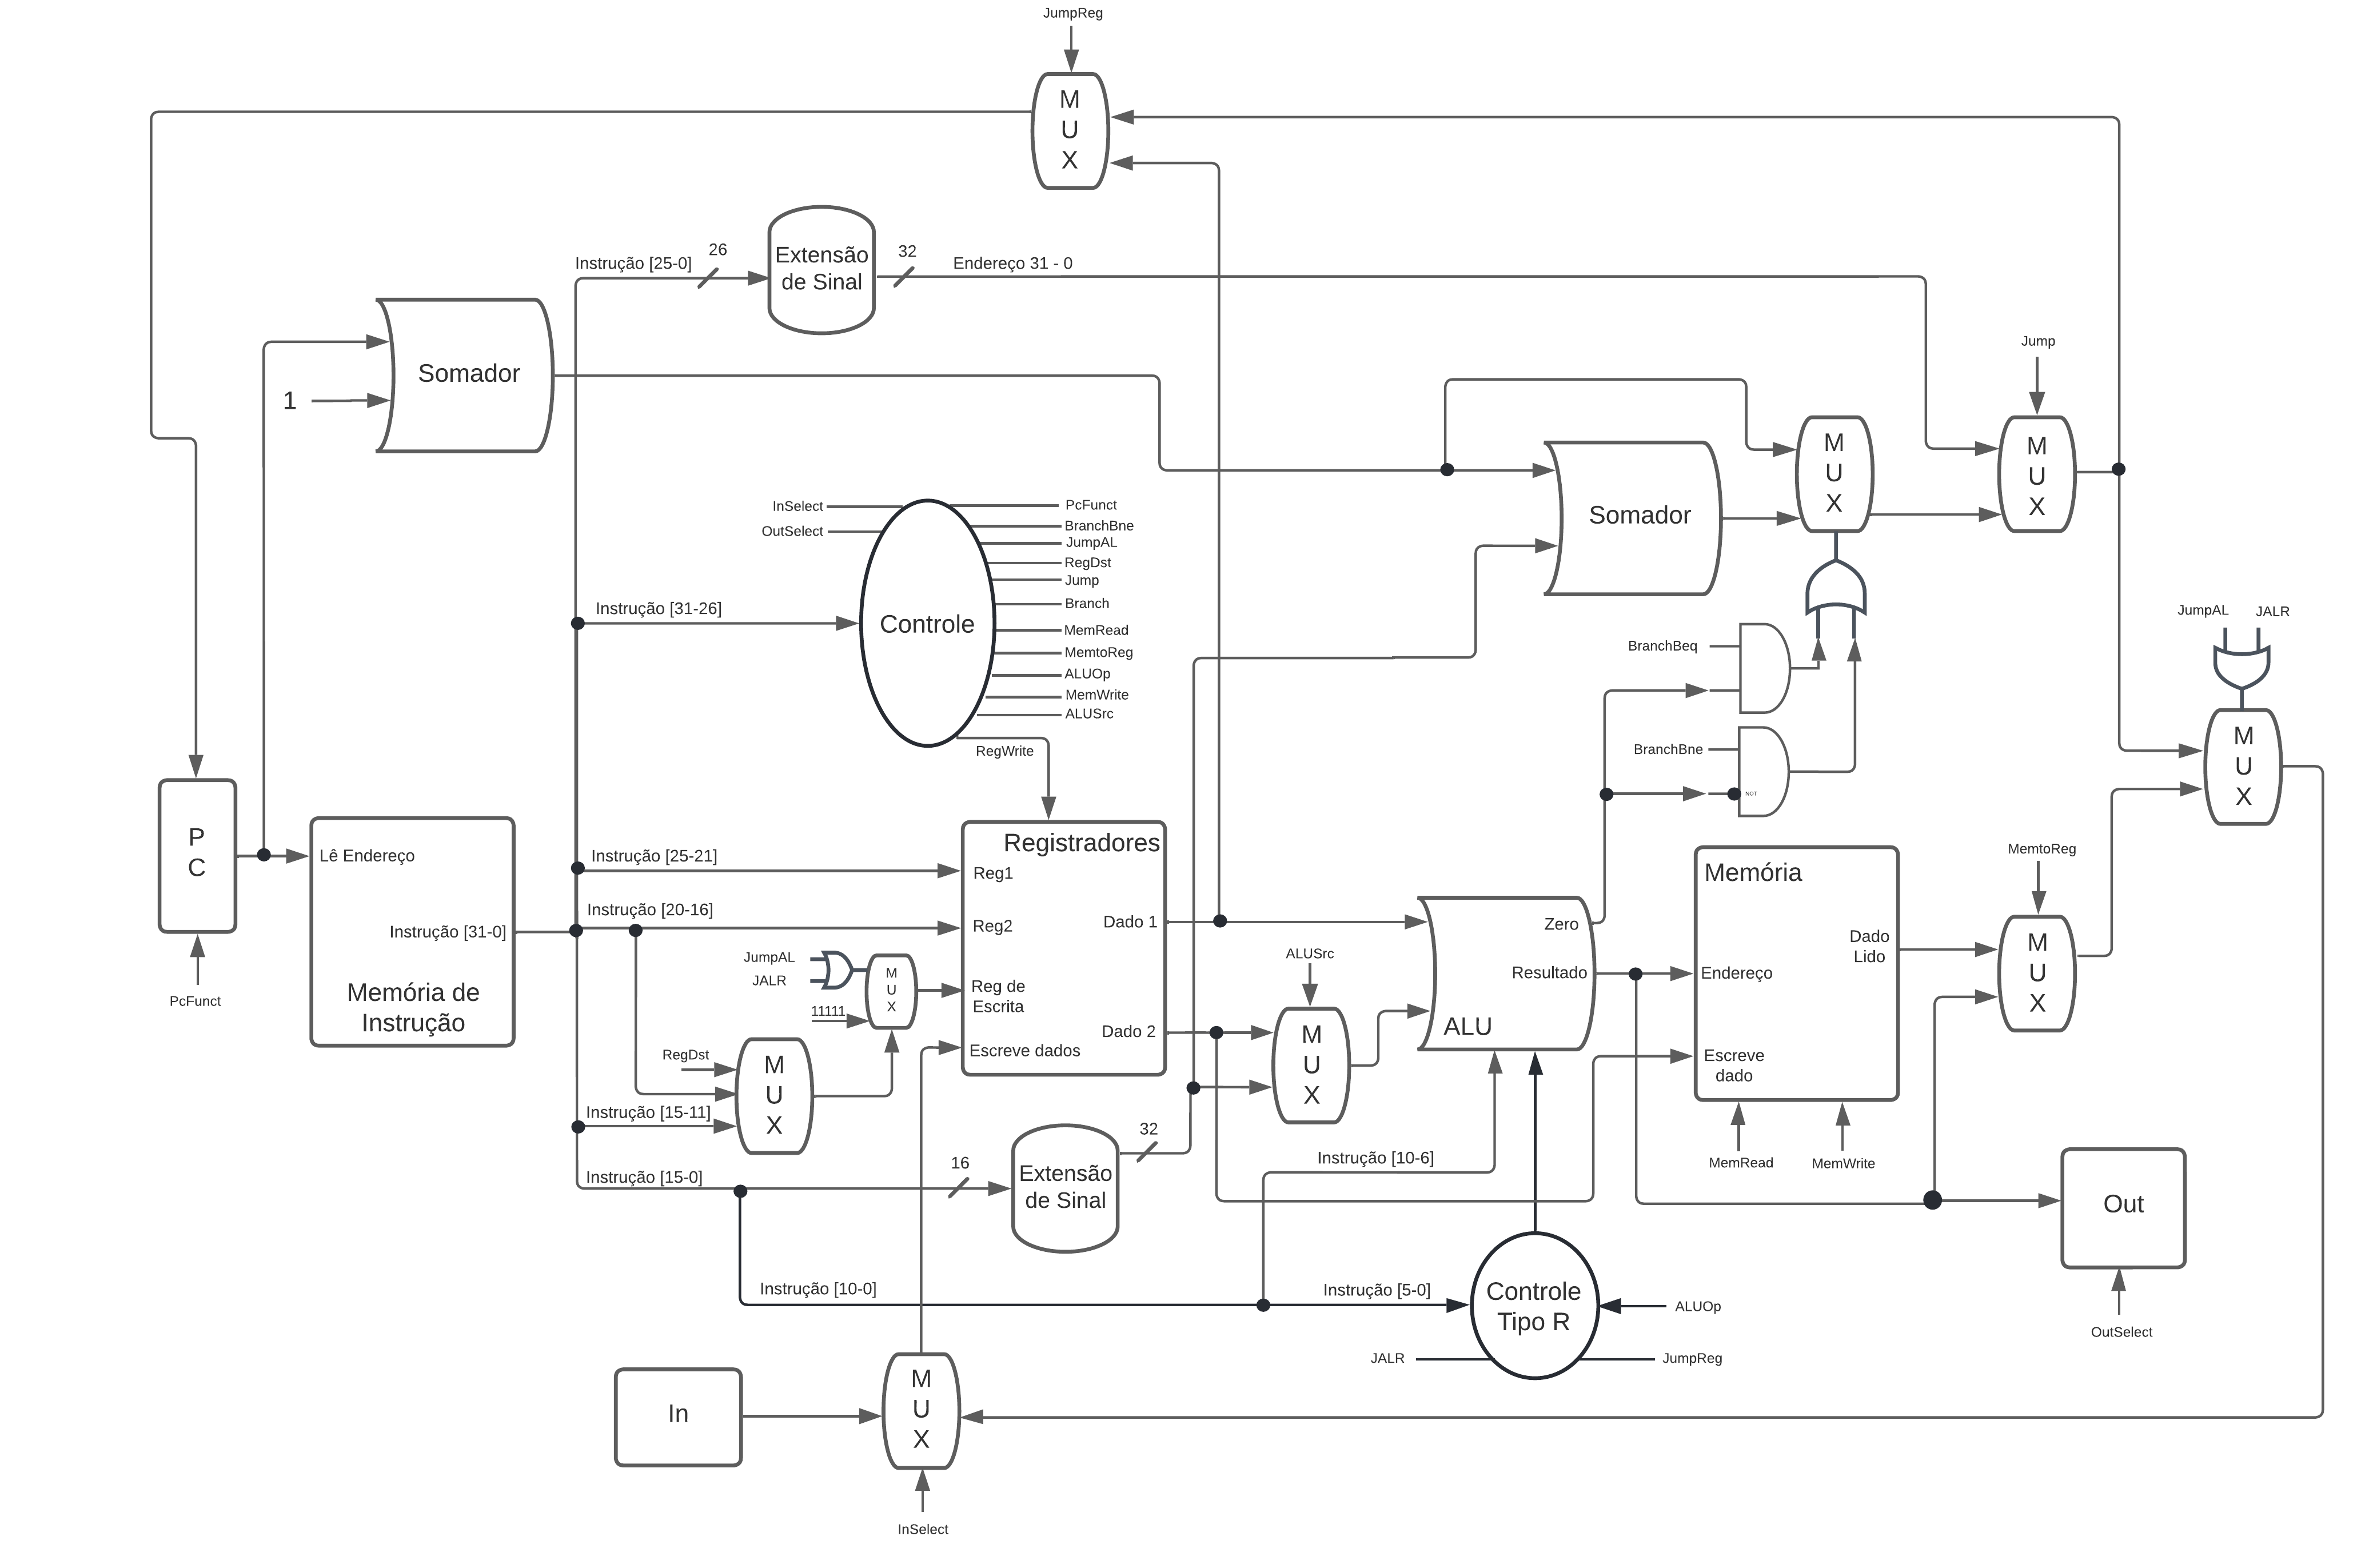
\includegraphics[scale=0.11]{Datapath_Alterado.png}
\legend{Fonte: O Autor }
\end{figure}

Nesse diagrama do processador é importante ressaltar alguns componentes que possuem maiores relevâncias para o projeto. Primeiramente, temos a memória de instrução, que sua única entrada será o valor vindo do registrador PC, indicando qual será a instrução que será enviada para os demais segmentos. Em seguida, essa saída será divida em diversos segmentos, em que cada parte será enviada a um componente diferente. Cada segmento será um dos campos dos tipos de instruções. 

O banco de registradores irá possuir cinco entradas distintas, sendo elas: o endereço do primeiro registrador de entrada (rs); o endereço do segundo registrador de entrada (rt); o endereço do registrador de destino (rd ou rt); o dado a ser escrito em um dos registradores; e um bit de controle, para ativar e desativar a escrita no banco. Já as saídas serão os valores armazenados nos registradores indicados nos endereços de entrada.

As duas saídas do banco de registradores serão enviadas diretamente para a unidade lógica e aritmética, em que servirão como valores de entrada para realizar alguma de suas operações. Ademais, o valor da segunda entrada também poderá ser o valor de um imediato de 16bits de uma instrução do tipo I. Este valor deverá ser estendido para 32bits para que seja possível realizar sua operação na ULA. Além disso, temos mais duas outras entradas: o valor do ``shamt'' da instrução do tipo R e os \emph{bits} de controle, que dirão qual instrução será realizada. Como saída, será enviada por um cabo o valor do resultado obtido pela operação. Um outro bit também será emitido caso a resposta seja zero ou não.

Por fim, temos a memória principal. Ela recebe como entrada: o resultado do ULA, que será o endereço do dado a ser lido ou armazenado; o valor do dado a ser armazenado; e dois \emph{bits} de controle, sendo eles um para escrita e um para leitura dos dados. Como saída, ele emite o valor do dado desejado, que será armazenado no banco de registradores.

Ao realizar as instruções, o fluxo a ser realizado será sequencial, ou seja, da mesma maneira em que elas foram dispostas na memória de instruções. Porém, caso seja realizada uma instrução de pulo condicional ou incondicional, o valor do endereço obtido será encaminhado ao registrador PC e ele será atualizado. Dessa forma, é possível alterar a ordem em que as instruções serão efetuadas dentro do processador projetado. 

\section{Formato de Instruções}
Para transmitir uma instrução para o processador, é preciso possuir uma série de sinais eletrônicos altos e baixos, que em binário são representados com os números 1 e 0, respectivamente \cite{patterson2017}. Cada valor unitário do sistema binário é chamado de bit. O conjunto desses números formam as instruções, que serão interpretadas pelo processador. A partir disso, são selecionados campos específicos desses números para passarem informações importantes. Esses segmentos terão informações diferentes dependendo de qual instrução será realizada e o seu valor irá impactar de alguma forma o funcionamento geral do que será efetuado.

Dessa forma, o processador implementa a arquitetura RISC (\emph{Reduced Instruction Set Computer}) de 32 \emph{bits} e, consequentemente,  possui o mesmo número de \emph{bits} para todos os formatos de instruções.

O MIPS possui apenas três tipos de instruções diferentes, sendo eles: registrador (R); imediato (I); e de desvio incondicional (J). Cada um deles será segmentado de forma a armazenar informações diferentes. Na \autoref{tab:FormatInstrTypeR} é possível verificar as segmentações para o formato para o tipo R.

\begin{table}[H]
\centering
\ABNTEXfontereduzida
\caption{Formato de Instruções do tipo R} \label{tab:FormatInstrTypeR}
\begin{tabular}{r|p{1.7cm}|p{1.7cm}|p{1.7cm}|p{1.7cm}|p{1.7cm} | p{1.5cm}} 
\textbf{Tamanho (bits)} & 6 & 5 & 5 & 5 & 5 & 6 \\ \hline
\textbf{Campo} & OPcode & Reg1 (rs) & Reg2 (rt) & Reg3 (rd) & Shamt & Funct \\ \hline
\textbf{Bits} & 31 - 26 & 25 - 21 & 20 - 16 & 15 - 11 & 10 - 6 & 5 - 0\\
\end{tabular}
\legend{Fonte: O Autor}
\end{table}

O campo ``opcode'' indica ao processador a operação básica da instrução, segmento que será importante para os três tipos de instruções. Sem essa informação, não é possível diferenciar as instruções uma das outras. Essa informação é encaminhada para a unidade de controle, em que irá selecionar quais funcionalidades deverão ser ativadas ou desativadas para que a instrução seja efetuada corretamente. Além disso, o campo ``funct'' também servirá para o propósito de controle, porém voltado apenas para a unidade lógica e aritmética, escolhendo qual operação deverá ser realizada.

Ademais, temos três campos para armazenar o endereço de um dos registradores, sendo eles o primeiro registrador de origem (rs), o segundo registrador de origem (rt) e o registrador de destino (rd). Então, ao realizar uma operação entre ``rs'' e ``rt'', o valor final será armazenado em ``rd''. 

Por fim, temos o campo ``shamt'', que possui o propósito de realizar instruções que envolvam deslocar valores de \emph{bits}. Esse deslocamento pode ser realizado para a esquerda ou para a direita, dependendo de qual função será utilizada.

\begin{table}[H]
\centering
\ABNTEXfontereduzida
\caption{Formato de Instruções do tipo I} \label{tab:FormatInstrTypeI}
\begin{tabular}{r|p{1.7cm}|p{1.7cm}|p{1.7cm}|p{1.7cm}} 
\textbf{Tamanho (bits)} & 6 & 5 & 5 & 16 \\ \hline
\textbf{Campo} & OPcode & Reg1 (rs) & Reg2 (rt) & Imediato \\ \hline
\textbf{Bits} & 31 - 26 & 25 - 21 & 20 - 16 & 15 - 0\\
\end{tabular}
\legend{Fonte: O Autor}
\end{table}

Na \autoref{tab:FormatInstrTypeI} está ilustrado o formato de instrução para o tipo I. É possível verificar que as únicas diferenças para o tipo R seriam que os campos ``rd'', ``shamt'' e ``funct'' foram alterados para comportar um imediato de 16 \emph{bits}. Esse imediato pode possuir diversas funções, seja para suportar um endereço de memória ou um valor para realizar uma operação aritmética.

Em determinadas instruções do tipo I, será preciso acessar ou armazenar dados em registradores. Assim, ``rs'' será o registrador para leitura das informações e ``rt'' o registrador destino. 


\begin{table}[H]
\centering
\ABNTEXfontereduzida
\caption{Formato de Instruções do tipo J} \label{tab:FormatInstrTypeJ}
\begin{tabular}{r|p{1.7cm}|p{1.7cm}} 
\textbf{Tamanho (bits)} & 6 & 26 \\ \hline
\textbf{Campo} & OPcode & Imediato \\ \hline
\textbf{Bits} & 31 - 26 & 25 - 0\\
\end{tabular}
\legend{Fonte: O Autor}
\end{table}

Por último, na \autoref{tab:FormatInstrTypeJ}, o formato de instruções para o tipo I. Neste, os únicos campos existentes será o \emph{opcode} e o imediato de 26 \emph{bits}. Esse imediato será importante para armazenar o endereço de uma instrução na memória de instruções, permitindo que seja possível realizar desvios incondicionais.

\section{Conjunto de Instruções}
Com os formatos definidos no seção anterior, é possível descrever quais serão as instruções que serão implementadas para esse processador. Dessa forma, nas Tabelas \ref{tab:InstrR}, \ref{tab:InstrI} e \ref{tab:InstrJ} estão representadas essas instruções, em conjunto com os seus nomes, números de identificação e qual a sua funcionalidade.


\begin{table}[H]
\centering
\ABNTEXfontereduzida
\caption{Instruções do tipo R} \label{tab:InstrR}
\begin{tabular}{||c c c c||} 
 \hline
 OPcode & Funct & Nome & Função \\ [0.5ex] 
 \hline\hline
 000000 & 100000 & ADD & rd ← rs + rt \\ 
 \hline
 000000 & 100010 & SUB & rd ← rs - rt \\
 \hline
 000000 & 100100 & AND & rd ← rs \& rt \\
 \hline
 000000 & 100101 & OR & rd ← rs | rt \\
 \hline
 000000 & 101101 & XOR & rd ← rs $\oplus$ rt \\
 \hline
 000000 & 001000 & JR & PC ← rs  \\  
 \hline
 000000 & 001001 & JALR & ra ← endereço; PC ← rs \\  
 \hline
 000000 & 101010 & SLT & rd ← (rs < rt); 0 se falso; 1 se verdadeiro\\  
 \hline
 000000 & 100111 & NOR & rd ← rs $\sim|$ \  rt \\
 \hline
 000000 & 000000 & SLL & rd ← rt << shamt \\ 
 \hline
 000000 & 000010 & SRL & rd ← rt >> shamt \\
 \hline
 000000 & 011010 & DIV & rd ← rs / rt \\
 \hline
 000000 & 011000 & MULT & rd ← rs * rt \\
 \hline
\end{tabular}
\legend{Fonte: O Autor}
\end{table}


\begin{table}[H]
\centering
\ABNTEXfontereduzida
\caption{Instruções do tipo I} \label{tab:InstrI}
\begin{tabular}{||c c c||} 
 \hline
 OPcode &  Nome & Função \\ [0.5ex] 
 \hline\hline
 100011 & LW & rt ← Mem[ base + offset ]  \\ 
 \hline
 101011 & SW & Mem[ base + offset ] ← rt \\
 \hline
 001000 & ADDI & rt ← rs + Imm \\
 \hline
 001001 & SUBI & rt ← rs - Imm \\
 \hline
 001100 & ANDI & rt ← rs \& Imm \\
 \hline
 001101 & ORI & rt ← rs | Imm \\
 \hline
 101101 & XORI & rt ← rs $\oplus$ Imm \\
 \hline
 000100 & BEQ & Se (rs == rt) então branch  \\  
 \hline
 000101 & BNE & Se (rs != rt) então branch \\  
 \hline
 001010 & SLTI & rt ← (rs < Imm); 0 se falso; 1 se verdadeiro \\ 
 \hline
 011111 & IN & rt ← Imm \\
 \hline
 011110 & OUT & saída ← rs \\
 \hline
\end{tabular}
\legend{Fonte: O Autor}
\end{table}

\begin{table}[H]
\centering
\ABNTEXfontereduzida
\caption{Instruções do tipo J} \label{tab:InstrJ}
\begin{tabular}{||c c c||} 
 \hline
 OPcode & Nome & Função \\ [0.5ex] 
 \hline\hline
 000010 & J & Jump para o endereço \\ 
 \hline
 000011 & JAL & ra ← PC + 1; Jump para o endereço \\
 \hline
 111111 & HALT & Parar o processador \\
 \hline
\end{tabular}
\legend{Fonte: O Autor}
\end{table}

\section{Modos de Endereçamento}
Os meios de acesso aos operandos das instruções são chamados de modos de endereçamento, que são salvos na memória do processador, seja na memória principal, de instrução ou o banco de registradores \cite{patterson2006}. Em uma arquitetura MIPS, existem cinco modos de endereçamentos, porém na implementação do projeto foram utilizados apenas quatro delas, que serão explicadas a seguir.
	
\subsection{A Registrador}
Neste primeiro modo de endereçamento temos que, em um dos segmentos da instrução, existirá um termo que indicará o endereço de um registrador no banco de registradores e, assim, podemos obter o operando armazenado dentro dele. É possível observar que na instrução do tipo R (\autoref{tab:FormatInstrTypeR}) será passado o endereço de três registradores (rs, rt e rd). Já nas instruções do tipo I (\autoref{tab:FormatInstrTypeI}) temos apenas dois endereços (rs e rt).

\subsection{Imediato}
Neste caso, teremos que o endereço de um certo operando na memória principal será referenciado por um valor imediato, com um valor máximo de 16bits. O único tipo de instrução a utilizar esse modo será a do tipo I (\autoref{tab:FormatInstrTypeI}), que possuí um campo justamente para esse valor imediato.

\subsection{Base-Deslocamento}
Para esse tipo, o valor do endereço a ser escolhido na memória principal será relativo a um vetor. Ou seja, utilizamos um valor como base, que será o inicio do vetor, e depois deslocamos uma quantidade de \emph{bits} para encontrar a posição desejada nesta lista. É um modo de endereçamento utilizado por instruções de \emph{load} e \emph{store}, que são do tipo I (\autoref{tab:FormatInstrTypeI}), em que o valor armazenado em ``rs'' será o valor base e o imediato o valor do deslocamento.

\subsection{Absoluto}
Para finalizar, o último modo, da mesma forma que o relativo ao PC, também influência apenas na memória de instrução. Neste caso, o valor do endereço é totalmente passado pelo imediato de 26 \emph{bits}. Dizemos que ele é absoluto por ser o maior valor possível que podemos passar por meio de uma instrução, já que os demais 6 \emph{bits} são destinados ao opcode. Dessa forma, para indicar isso, ele também pode ser chamado de pseudo-absoluto. o único tipo de instrução capaz de realizar esse modo de endereçamento é a do tipo J (\autoref{tab:FormatInstrTypeJ}).


\chapter{Compilador para a linguagem C-}

Como qualquer outro software, um compilador de uma nova linguagem deve, preferencialmente, ser escrito em uma linguagem de programação que já possua um compilador ou interpretador implementado, para que assim seja possível obter todos os benefícios de se trabalhar com uma linguagem de alto nível. Nesse projeto, a linguagem de programação escolhido foi a C.

\section{Fase de Análise}

A fase de análise é o momento em que o compilador irá analisar se o que foi escrito pelo programador está coerente com as regras propostas pela linguagem. Caso algum erro tenha sido cometido, o compilador deve avisá-lo e parar seus procedimentos, sem continuar para a fase de síntese, para que assim o programador possa arrumá-los.

\subsection{Modelagem}

\subsubsection{Diagrama de Blocos}

\begin{figure}[H]
\centering 
\caption{Diagrama de blocos para a fase de análise} \label{fig:DiagramaBlocosAnalise}
\graphicspath{ {./imgs/} } 
\includegraphics[scale=0.3]{imgs/Diagrama de Blocos Fase Análise.jpg}
\legend{Fonte: O Autor }
\end{figure}

\subsubsection{Diagrama de Atividades}

\begin{figure}[H]
\centering 
\caption{Diagrama de atividades para a fase de análise} \label{fig:DiagramaAtividadesAnalise}
\graphicspath{ {./imgs/} } 
\includegraphics[scale=0.35]{imgs/Diagrama de Atividades Fase de Análise.jpg}
\legend{Fonte: O Autor }
\end{figure}

\subsection{Análise Léxica}

A análise léxica é a primeira verificação que todo compilador irá realizar. Sua importância é encontrar os ``tokens'' da linguagem, ou seja, se as palavras colocadas no código são de alguma forma interpretadas pelo compilador e, em caso afirmativo, agrupá-las em seu significado geral. Caso um simbolo ou palavra não for reconhecido pelo analisador, um erro léxico deverá ocorrer.

Os símbolos com os seus respectivos tokens podem ser observados na \autoref{tab:Tokens}.

\begin{table}[H]
\centering
\ABNTEXfontereduzida
\caption{Relação entre símbolos e tokens para o compilador} \label{tab:Tokens}
\begin{tabular}{||c c||} 
 \hline
 Simbolo & Token\\ [0.5ex] 
 \hline\hline
 Números (0-9) & NUM \\ 
 \hline
 Nomes de Variáveis/Funções & ID \\
 \hline
 void  &  VOID\\
 \hline
 if  &  IF\\
 \hline
 int  &  INT\\
 \hline
 else  &  ELSE\\
 \hline
 return  &  RETURN\\
 \hline
 while  &  WHILE\\
 \hline
 (  &  ABREPARENTESES\\
 \hline
 )  &  FECHAPARENTESES\\
 \hline
 [  &  ABRECOLCHETES\\
 \hline
 ]  &  FECHACOLCHETES\\
 \hline
 \{  &  ABRECHAVES\\
 \hline
 \}  &  FECHACHAVES\\
 \hline
 =  &  ATRIB\\
 \hline
 ,  &  COMMA\\
 \hline
 ;  &  SEMICOLON\\
 \hline
 +  &  SOMA\\
 \hline
 -  &  SUB\\
 \hline
 *  &  MULT\\
 \hline
 ==  &  EQ\\
 \hline
 !=  &  NEQ\\
 \hline
 <  &  LT\\
 \hline
 >  &  GT\\
 \hline
 <=  &  LET\\
 \hline
 >=  &  GET\\
 \hline
 Diferente dos símbolos acima  &  ERRO\\
 \hline
\end{tabular}
\legend{Fonte: O Autor}
\end{table}


\subsection{Análise Sintática}

O analisador sintático tem a função de verificar se o que foi escrito pelo programador está coeso, ou seja, se os tokens estão em uma ordem possível de se ocorrer. Essa verificação é importante por manter regras que permitem o compilador linearizar o código escrito em um código sequencial, que será facilmente entendido pelo processador. Caso um token encontrado não esteja definido para estar presentes naquele momento, um erro sintático devera ser apresentado para o usuário.

As regras da análise sintática são definidas por gramaticas livre de contexto (CFG). Cada linguagem de programação possui a sua gramatica definida a priori pelos desenvolvedores do compilador. Dessa forma, na \autoref{tab:CFG} é possível verificar a gramática definida para linguagem C-. 

\begin{table}
\centering
\ABNTEXfontereduzida
\caption{Sintaxe da linguagem C- utilizada no projeto\\ } \label{tab:CFG}
\resizebox{\linewidth}{!}{%
\begin{tabular}{|l|l|}  \hline \\
\vcell{programa} & \vcell{declaracao\_lista} \\[-\rowheight]
\printcelltop & \printcelltop \\ \hline
\multirow{2}{*}{declaracao\_lista} & \vcell{declaracao\_lista declaracao} \\[-\rowheight]
 & \printcelltop \\ \cline{2-2}
 & \vcell{declaracao} \\[-\rowheight]
 & \printcelltop \\ \hline
\multirow{2}{*}{declaracao} & \vcell{var\_declaracao} \\[-\rowheight]
 & \printcelltop \\ \cline{2-2}
 & \vcell{fun\_declaracao} \\[-\rowheight]
 & \printcelltop \\ \hline
\multirow{2}{*}{var\_declaracao} & \vcell{tipo\_especificador ID SEMICOLON} \\[-\rowheight]
 & \printcelltop \\ \cline{2-2}
 & \vcell{tipo\_especificador ID ABRECOLCHETES NUM FECHACOLCHETES SEMICOLON} \\[-\rowheight]
 & \printcelltop \\ \hline
\multirow{2}{*}{tipo\_especificador} & \vcell{INT} \\[-\rowheight]
 & \printcelltop \\ \cline{2-2}
 & \vcell{VOID} \\[-\rowheight]
 & \printcelltop \\ \hline
\vcell{fun\_declaracao} & \vcell{tipo\_especificador fun\_id ABREPARENTESES params FECHAPARENTESES composto\_decl} \\[-\rowheight]
\printcelltop & \printcelltop \\ \hline
\vcell{fun\_id} & \vcell{ID} \\[-\rowheight]
\printcelltop & \printcelltop \\ \hline
\multirow{2}{*}{params} & \vcell{param\_lista} \\[-\rowheight]
 & \printcelltop \\ \cline{2-2}
 & \vcell{VOID} \\[-\rowheight]
 & \printcelltop \\ \hline
\multirow{2}{*}{param\_lista} & \vcell{param\_lista COMMA param} \\[-\rowheight]
 & \printcelltop \\ \cline{2-2}
 & \vcell{param} \\[-\rowheight]
 & \printcelltop \\ \hline
\multirow{2}{*}{param} & \vcell{tipo\_especificador ID} \\[-\rowheight]
 & \printcelltop \\ \cline{2-2}
 & \vcell{tipo\_especificador ID ABRECOLCHETES FECHACOLCHETES} \\[-\rowheight]
 & \printcelltop \\ \hline
\vcell{composto\_decl} & \vcell{ABRECHAVES local\_declaracoes statement\_lista FECHACHAVES} \\[-\rowheight]
\printcelltop & \printcelltop \\ \hline
\vcell{local\_declaracoes} & \vcell{local\_declaracoes var\_declaracao \textbar{} \%empty} \\[-\rowheight]
\printcelltop & \printcelltop \\ \hline
\vcell{statement\_lista} & \vcell{statement\_lista statement \textbar{} \%empty} \\[-\rowheight]
\printcelltop & \printcelltop \\ \hline
\multirow{5}{*}{statement} & \vcell{expressao\_decl} \\[-\rowheight]
 & \printcelltop \\ \cline{2-2}
 & \vcell{composto\_decl} \\[-\rowheight]
 & \printcelltop \\ \cline{2-2}
 & \vcell{selecao\_decl} \\[-\rowheight]
 & \printcelltop \\ \cline{2-2}
 & \vcell{iteracao\_decl} \\[-\rowheight]
 & \printcelltop \\ \cline{2-2}
 & \vcell{retorno\_decl} \\[-\rowheight]
 & \printcelltop \\ \hline
\multirow{2}{*}{expressao\_decl} & \vcell{expressao SEMICOLON} \\[-\rowheight]
 & \printcelltop \\ \cline{2-2}
 & \vcell{SEMICOLON} \\[-\rowheight]
 & \printcelltop \\ \hline
\vcell{selecao\_decl} & \vcell{IF ABREPARENTESES expressao FECHAPARENTESES statement fatoracao} \\[-\rowheight]
\printcelltop & \printcelltop \\ \hline
\vcell{fatoracao} & \vcell{ELSE statement \textbar{} \%empty} \\[-\rowheight]
\printcelltop & \printcelltop \\ \hline
\vcell{iteracao\_decl} & \vcell{WHILE ABREPARENTESES expressao FECHAPARENTESES statement} \\[-\rowheight]
\printcelltop & \printcelltop \\ \hline
\multirow{2}{*}{retorno\_decl} & \vcell{RETURN SEMICOLON} \\[-\rowheight]
 & \printcelltop \\ \cline{2-2}
 & \vcell{RETURN expressao SEMICOLON} \\[-\rowheight]
 & \printcelltop \\ \hline
\multirow{2}{*}{expressao} & \vcell{var ATRIB expressao} \\[-\rowheight]
 & \printcelltop \\ \cline{2-2}
 & \vcell{simples\_expressao} \\[-\rowheight]
 & \printcelltop \\ \hline
\multirow{2}{*}{var} & \vcell{ID} \\[-\rowheight]
 & \printcelltop \\ \cline{2-2}
 & \vcell{ID ABRECOLCHETES expressao FECHACOLCHETES} \\[-\rowheight]
 & \printcelltop \\ \hline
\multirow{2}{*}{simples\_expressao} & \vcell{soma\_expressao relacional soma\_expressao} \\[-\rowheight]
 & \printcelltop \\ \cline{2-2}
 & \vcell{soma\_expressao} \\[-\rowheight]
 & \printcelltop \\ \hline
\vcell{relacional} & \vcell{operador\_relacional} \\[-\rowheight]
\printcelltop & \printcelltop \\ \hline
\vcell{operador\_relacional} & \vcell{EQ \textbar{} NEQ \textbar{} LT \textbar{} GT \textbar{}  LET \textbar{} GET} \\[-\rowheight]
\printcelltop & \printcelltop \\ \hline
\multirow{2}{*}{soma\_expressao} & \vcell{soma\_expressao soma termo} \\[-\rowheight]
 & \printcelltop \\ \cline{2-2}
 & \vcell{termo} \\[-\rowheight]
 & \printcelltop \\ \hline
\vcell{soma} & \vcell{SOMA \textbar{} SUB} \\[-\rowheight]
\printcelltop & \printcelltop \\ \hline
\multirow{2}{*}{termo} & \vcell{termo mult fator} \\[-\rowheight]
 & \printcelltop \\ \cline{2-2}
 & \vcell{fator} \\[-\rowheight]
 & \printcelltop \\ \hline
\vcell{mult} & \vcell{MULT \textbar{} DIV} \\[-\rowheight]
\printcelltop & \printcelltop \\ \hline
\multirow{4}{*}{fator} & \vcell{ABREPARENTESES expressao FECHAPARENTESES} \\[-\rowheight]
 & \printcelltop \\ \cline{2-2}
 & \vcell{var} \\[-\rowheight]
 & \printcelltop \\ \cline{2-2}
 & \vcell{ativacao} \\[-\rowheight]
 & \printcelltop \\ \cline{2-2}
 & \vcell{NUM} \\[-\rowheight]
 & \printcelltop \\ \hline
\vcell{ativacao} & \vcell{fun\_id ABREPARENTESES args FECHAPARENTESES} \\[-\rowheight]
\printcelltop & \printcelltop \\ \hline
\vcell{args} & \vcell{arg\_lista \textbar{} \%empty} \\[-\rowheight]
\printcelltop & \printcelltop \\ \hline
\multirow{2}{*}{arg\_lista} & \vcell{arg\_lista COMMA expressao} \\[-\rowheight]
 & \printcelltop \\ \cline{2-2}
 & \vcell{expressao} \\[-\rowheight]
 & \printcelltop \\ \hline
\end{tabular}
}
\legend{Fonte: O Autor}
\end{table}


Ao verificar as regras da gramática, o compilador realiza a geração de uma estrutura muito relevantes para as fases seguintes do projeto, chamada de árvore de analise sintática. Ela é uma estrutura do tipo árvore que cada nó pode possuir um irmão e no máximo três filhos, dessa forma cada um deverá representar alguma informação relevante sobre o que o programador está fazendo naquele momento, como por exemplo: declaração de variáveis e funções, operações aritméticas, utilização das variáveis e demais outras. Sem essa estrutura, não seria possível realizar a análise seguinte e a geração do código intermediário, já que as duas precisam percorre-la para extrair as informações necessárias.

\subsection{Análise Semântica}

Caso o código não possua erros após as duas verificações anteriores, então concluímos que ele está escrito corretamente e padronizado nas regras da linguagem, ou seja, não viola sua sintaxe. Porém, ainda assim é possível que essas expressões não façam sentido ou estejam logicamente incorretas, o que poderia ocasionar em um comportamento anormal do código fonte, caso eles não fossem alterados. Esses erros dependem do projetista da linguagem, já que eles podem estar presentes em uma e não em outra.

Na linguagem de programação C- os erros semânticos são semelhantes aos da linguagem original C. Na \autoref{tab:Semantico} estão presentes os erros semânticos que foram tratados no projeto deste compilador e a explicação do que ele indica.


\begin{table}[H]
\centering
\ABNTEXfontereduzida
\caption{Erros semânticos presentes na linguagem C-} \label{tab:Semantico}
\begin{tabular}{||m{6cm} | |m{9cm}||} 
 \hline
\multicolumn{1}{||m{6cm}||}{\centering Erro} & \multicolumn{1}{m{9cm}||}{\centering Explicação}\\ [0.5ex] 
 \hline
 Declaração variável como void & Não é possível declarar uma variável do tipo void, já que seria de um tipo inexiste e não conseguiria ser usado pelo processador. \\ 
 \hline
 Declaração de função duplicada & Quando duas funções são nomeadas com o mesmo ID, impedindo o compilador de identificar qual a certa a ser chamada.  \\
 \hline
 Declaração de Variável duplicada & Quando duas variáveis, no mesmo escopo, estão definidas com o mesmo ID. \\
 \hline
 Declaração de função com nome de variável & Quando uma função é declarada, mas uma variável já possuía esse mesmo ID anteriormente. \\
 \hline
 Declaração de variável com nome de função & Quando uma variável é declarada, mas uma função já possuía esse mesmo ID anteriormente. \\
 \hline
 Variável não declarada & Quando uma variável é utilizada, mas ela não foi declarada. Isso impede o compilador de alocar um espaço na memória para aquela variável em questão. \\
 \hline
 Função não declarada & Ocorre quando uma função é utilizada sem ser declarada, impedindo o compilador de realizar o desvio do código fonte, já que ela não existe. \\
 \hline
 Atribuições de funções do tipo Void & Como funções declaradas com o tipo Void não retornam valores, não é possível realizar atribuições a variáveis com ela.\\
 \hline
 Função ``main'' não declarada & Caso essa função não exista, não existe um procedimento inicial para iniciar o código fonte. \\ 
 \hline
 Vetor não declarado & Quando uma variável é utilizada como vetor, mas ela não foi declarada.\\
 \hline
 Chamada de função não realizada & Quando o ID de uma função é escrito, porém não foi utilizado () no final do mesmo.\\
 \hline
\end{tabular}
\legend{Fonte: O Autor}
\end{table}

\section{Fase de Síntese}

Nesse momento, o compilador já realizou todas as verificações cabíveis e está pronto a iniciar a geração do código fonte. Caso algum erro tenha sido levantado na fase anterior, o compilador irá concluir sua execução, já que não faz sentido a geração de um código com erros envolvidos e cabe ao programador corrigi-los e realizar uma nova instância do programa. Essa fase é divida em três partes: código intermediário, código \emph{assembly} e código binário, que serão descritas nas próximas seções.

\subsection{Modelagem}

\subsubsection{Diagrama de Blocos}

\begin{figure}[H]
\centering 
\caption{Diagrama de blocos para a fase de síntese} \label{fig:DiagramaBlocosSintese}
\graphicspath{ {./imgs/} } 
\includegraphics[scale=0.3]{imgs/Diagrama de Blocos Codigo Intermediário.jpg}
\legend{Fonte: O Autor }
\end{figure}


\subsubsection{Diagrama de Atividades}

\begin{figure}[H]
\centering 
\caption{Diagrama de atividades para a fase de síntese} \label{fig:DiagramaAtividadesSintese}
\graphicspath{ {./imgs/} } 
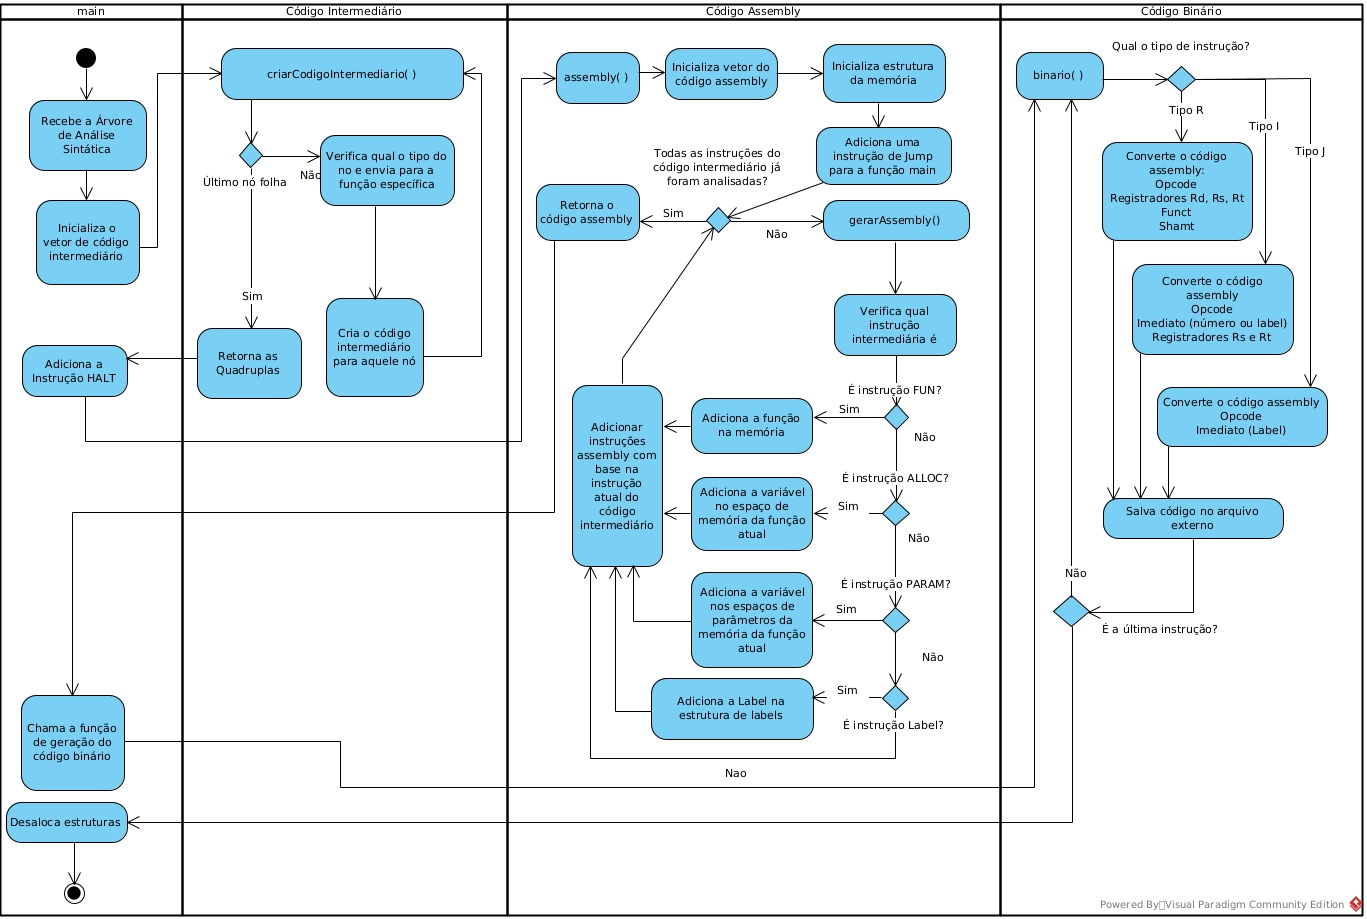
\includegraphics[scale=0.3]{imgs/Diagrama de Atividades Código Intermediário.jpg}
\legend{Fonte: O Autor }
\end{figure}


\subsection{Código Intermediário}

O código intermediário é o primeiro mecanismo após o código ter sido totalmente verificado na fase de análise. O seu principal propósito é transformar uma estrutura não linear em linear, que nesse caso, é o código escrito na linguagem C-, representado pela árvore de análise sintática, e transformada em pseudo instruções sequenciais.

Essas pseudo-instruções são generalizadas e podem representar diversos códigos de maquinas distintos. Isso é importante já que o compilador pode realizar esse procedimento até esse ponto para qualquer máquina, pois as instruções do código intermediário serão as mesmas. Dessa forma, caso o projetista do compilador queira realizar a geração do código \emph{assembly} diretamente, sem passar por essa fase em questão, não teria problema para aquela máquina em questão, porém seria mais complexo realizar a portabilidade daquele programa para demais máquinas.

Como visto anteriormente, a árvore de análise sintática é extremamente importante, pois é com ela que toda a estrutura do código fonte foi armazenado para indicar o que aquele código deve realizar. Assim, o gerador de código intermediário deve percorrer os nós da árvore e adicionar as instruções que realizam a operação desejada. Essas instruções foram descritas na \autoref{tab:CodigoIntermediario}.

\begin{table}[htb]
\centering
\ABNTEXfontereduzida
\caption{Instruções do código intermediário} \label{tab:CodigoIntermediario}
\begin{tabular}{||m{4cm} | |m{10cm}||} 
 \hline
\multicolumn{1}{||m{4cm}||}{\centering Pseudo-Instrução} & \multicolumn{1}{m{10cm}||}{\centering Explicação}\\ [0.5ex] 
 \hline \hline
 IFF & Uma instrução para verificar se o valor passado por ele é igual a 0. Em caso afirmativo, um desvio deve ser realizado para a label indicada (desvio condicional).\\ 
 \hline
 LABEL & Indica que deve existir uma label naquele ponto do código. Elas são utilizadas para marcações de pontos de interesse, em que o código pode realizar saltos condicionais ou incondicionais. Exemplos: nome de funções e finalização de uma função.  \\
 \hline
 GOTO & Realiza um desvio incondicional para a label indicada.\\
 \hline
 FUN & Indica o início de uma função. \\
 \hline
 END & Indica a finalização de uma função. \\
 \hline
 ARG & Indica quais são os argumentos que devem ser passados para essa função. \\
 \hline
 LOAD & Acessa a memória de dados para trazer o valor armazenado de uma variável para o registrador indicado (memória para registrador). \\
 \hline
 ALLOC & Realiza a alocação de uma nova variável no escopo daquela função (ou global).\\
 \hline
 RET & Realiza o retorno para a função acima na pilha, ou seja, a função anterior. \\ 
 \hline
 ADD - SUB - MULT - DIV & Realiza as operações aritméticas de soma, subtração, multiplicação e divisão, respectivamente.\\
 \hline
 LOADI & Salva o valor de um imediato inteiro dentro do registrador especificado.\\
 \hline
 EQ - NEQ - GT - LT - GET - LET & Realiza operações relacionais entre dois registradores, retornando verdadeiro (1) ou falso (0). Elas são: igualdade, não igualdade, maior que, menor que, maior ou igual que e menor ou igual que, respectivamente.\\
 \hline
 CALL & Realiza a chamada para a função indicada. \\
 \hline
 PARAM & Utilizado para passar parâmetros como argumentos de funções. Esses parâmetros devem ser enviados antes de realizar uma instrução de CALL.\\
 \hline
 ASSIGN & Realiza uma atribuição de valor para uma variável (registrador para registrador).\\
 \hline
 STORE & Armazena o dado da variável na memória de dados (registrador para a memória).\\
 \hline
\end{tabular}
\legend{Fonte: O Autor}
\end{table}


Primeiramente, é necessário a construção de uma estrutura de dados que consiga armazenar essas instruções e, dessa forma, as duas \emph{structs}, representadas na \autoref{fig:StructsCodInterm} foram criadas para tal. A \emph{struct} ``INSTRUCAO'' armazena o nome da operação a ser realizada em conjunto com os seus três argumentos, já que é valor máximo de argumentos que um código intermediário possui. Esses argumentos são armazenados em \emph{structs} chamadas ``ENDERECO'' utilizada, em que cada um pode ser do tipo \emph{string}, inteiro ou vazia (caso não possua valor). Por fim, todas as instruções são armazenadas no vetor ``codigoIntermediario''.

\afterpage{
\begin{figure}[htb]
\centering 
\caption{Estrutura de dados para o código intermediário, presente no arquivo \nohyphens{``codIterm.h''}} 
\label{fig:StructsCodInterm}
\graphicspath{ {./imgs/} } 
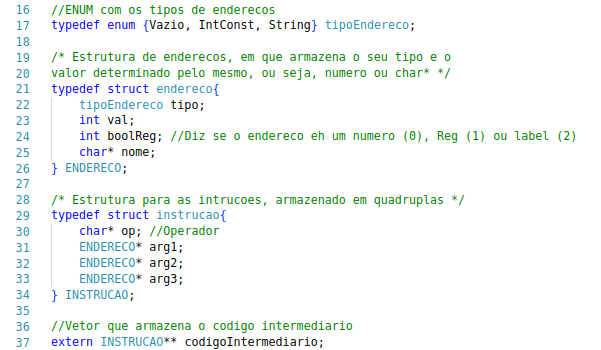
\includegraphics[scale=0.5]{Codigo/Struct_Codigo_Interm.png}
\legend{Fonte: O Autor }
\end{figure}
}

Assim, basta percorrer os nós da árvore e analisando o seus tipos, já que cada um corresponderá a uma instrução distinta. Além disso, os nós filhos também podem conter informações relevantes para aquela instrução, então isso deve ser levado em consideração ao ser criado o código intermediário. A \autoref{fig:GerarCodInterm} ilustra o código principal para a geração desse código, em que cada tipo irá possuir o seu próprio procedimento. Note que essa função é recursiva e, dessa forma, um nó pode chamar novamente a função ``criarCodigoIntermediario'' para percorrer os seus nós filhos. 

\begin{figure}[H]
\centering 
\caption{Função para gerar o código intermediário, com base nos possíveis nós da arvore sintática, no \nohyphens{``codIterm.c''}} 
\label{fig:GerarCodInterm}
\graphicspath{ {./imgs/} } 
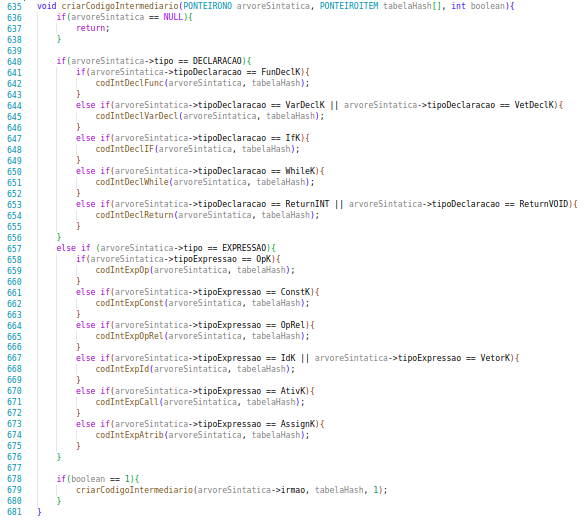
\includegraphics[scale=0.5]{imgs/Codigo/CodCriarCodInterm.png}
\legend{Fonte: O Autor }
\end{figure}


Para exemplificar esse procedimento, será descrito uma das funções utilizadas para a geração do código para exemplificar como as estruturas são criadas e o funcionamento da recursividade da passagem pelos nós. Na \autoref{fig:CodIntermOp} está ilustrado a função que cria o código intermediário para operadores aritméticos (soma, subtração, multiplicação e divisão) e, dessa forma, sempre que uma dessas operações seja encontrada na árvore de análise sintática, a função representada deve tratá-las. Dessa forma, a função primeiro verifica qual operação aritmética é, para poder atribuir o nome para a operação, com base na \autoref{tab:CodigoIntermediario}. 

\begin{figure}[H]
\centering 
\caption{Função para gerar o código intermediário ao encontrar um operador aritmético no \nohyphens{``codIterm.c''}} 
\label{fig:CodIntermOp}
\graphicspath{ {./imgs/} } 
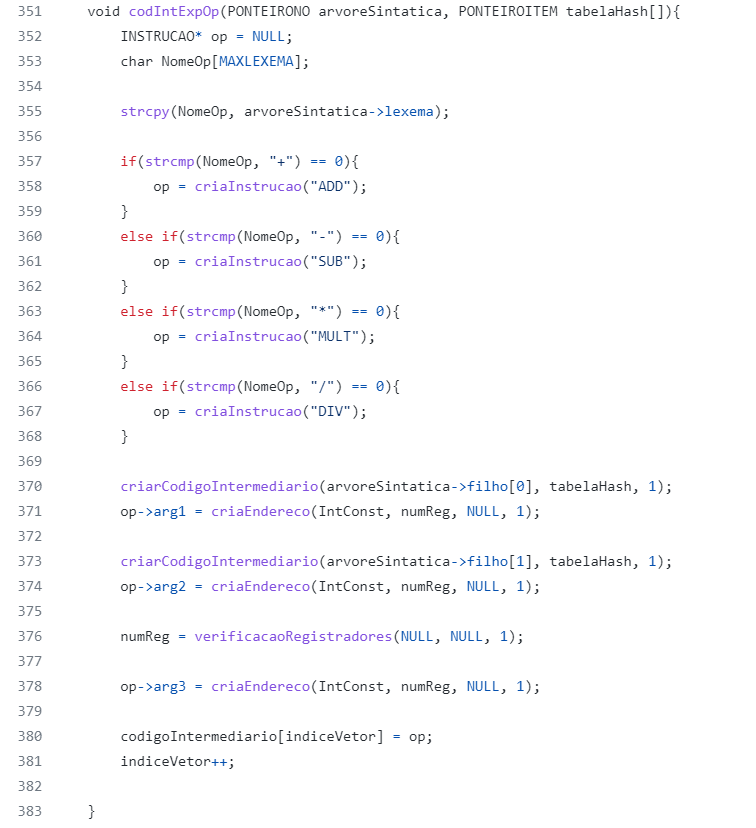
\includegraphics[scale=0.5]{imgs/Codigo/CodIntermOp.png}
\legend{Fonte: O Autor }
\end{figure}


A função ``criaInstrucao'' retorna uma \emph{struct} INSTRUCAO com todos os campos de argumentos vazios, permitindo que o programador decida posteriormente o que deve conter nesses espaços. Com isso, para o primeiro e segundo argumento, dois registradores devem ser utilizados para serem os operandos. Dessa maneira, antes é realizada uma chamada recursiva nos dois nós filhos, já que mais operações podem estar encadeadas, e seu registrador com o valor resultante das operações anteriores estará presente na variável global ``numReg'' e, dessa forma, basta colocar esse valor como argumento, por meio da função ``criaEndereco''. Por fim, é necessário escolher um registrador temporário que não esteja em uso no momento para poder armazenar o resultado da operação, por meio da instrução ``verificaRegistradores'', e armazenar o seu índice no terceiro argumento da instrução. Basta adicionar a nova instrução no vetor de código intermediário e incrementar o índice da próxima instrução.



\subsection{Código Assembly}

Diferentemente do código intermediário, a geração do código \emph{assembly} deve ser feito considerando as especificações da máquina alvo, já que cada processador possuí organizações e arquiteturas distintas que podem impactar em seu uso, como quantidade e tipos de instruções, números de registradores e quais possuem uso específico, especificações do acesso a memória e entre demais outras informações que devem ser levadas em consideração pelo programador do projeto. Nesse caso, a arquitetura e os tipos de instruções já foram descritas na seção anterior ``Processador MIPS''.

A geração é feita analisando cada instrução do código intermediário, traduzindo a sua funcionalidade para o código assembly da máquina, utilizando os três parâmetros como informações relevantes do que fazer a seguir. Cada código intermediário pode possuir uma ou mais instruções em código assembly para atingir o objetivo e funcionamento desejado (1 para N).

A estrutura desse código pode ser visualizada na \autoref{fig:StructsCodAssembly}, em que existem cinco \emph{structs} distintas, sendo três para cada tipo de instrução do código do processador (tipo R, I e J, respectivamente nas Tabelas \ref{tab:FormatInstrTypeR}, \ref{tab:FormatInstrTypeI}, \ref{tab:FormatInstrTypeJ}), outra para armazenar apenas valores de \emph{label} e, por fim, uma que possui uma instância de cada uma dentro dela, para poder ser criado uma lista única de código \emph{assembly} com os quatro tipos distintos descritos acima.


\begin{figure}[htb]
\centering 
\caption{Estrutura para armazenar o código assembly gerado, presente no arquivo \nohyphens{``assembly.h''}} 
\label{fig:StructsCodAssembly}
\graphicspath{ {./imgs/} } 
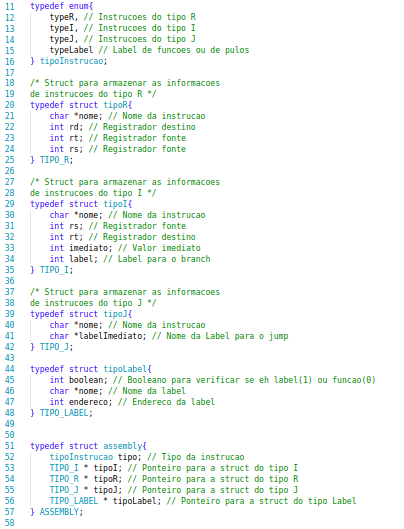
\includegraphics[scale=0.4]{imgs/Codigo/Struct_Codigo_Assembly.png}
\legend{Fonte: O Autor }
\end{figure}

Ademais, o processador possui internamente 32 registradores, porém alguns deles são reservados para uso específico do compilador. Eles estão descritos na \autoref{tab:Registradores} em conjunto com o seu nome e sua motivação de uso.

\begin{table}[htbp]
\centering
\ABNTEXfontereduzida
\caption{Valores dos registradores reservados e de uso geral do programa e do compilador} 
\label{tab:Registradores}
\begin{tabular}{||m{3cm}||m{2cm}||m{3.5cm}||m{5cm}||} 
\hline
\multicolumn{1}{||m{3cm}||}{\centering Registradores} & \multicolumn{1}{m{2cm}||}{\centering Número} & \multicolumn{1}{m{3.5cm}||}{\centering Nome} & \multicolumn{1}{m{5cm}||}{\centering Uso}\\ [0.5ex] 
 \hline \hline
\$zero  & 31 & Zero & Armazena sempre o valor 0 \\ \hline
\$ra   &  30 & Return Adress  & Armazena o endereço de retorno após uma chamada \\ \hline 
\$fp   & 29 & Frame Pointer & Armazena o índice do início da memória de dados daquela função em específico  \\ \hline 
\$sp   & 28 & Stack Pointer &  Armazena o índice do fim da memória de dados daquela função em específico     \\ \hline 
\$temp & 27 & Temporário & Registrador temporário para uso do compilador \\ \hline 
\$pilha  & 26 & Ponteiro para Pilha de parâmetros & Ponteiro para a região da pilha de parâmetros \\ \hline      
\$t0 - \$t25 & 0 - 25 & Registradores Diversos & Registradores para uso das operações do programa \\ \hline 
\end{tabular}
\legend{Fonte: O Autor }
\end{table}

Além disso, foi preciso criar uma estrutura capaz de gerenciar a memória da pilha de funções, já que será nela que dados importantes serão armazenados para aquele escopo em específico. Essa estrutura está ilustrada na \autoref{fig:StructsMemoria}. Cada função terá a possibilidade de armazenar até 25 valores inteiros de 32 bits dentro da memória, com alguns índices já pré selecionados para armazenar informações importantes para o compilador. A \autoref{tab:Memoria} representa um exemplo para uma função genérica.

\begin{table}[htb]
\centering
\ABNTEXfontereduzida
\caption{Tabela para a memória da pilha de funções} 
\label{tab:Memoria}
\begin{tabular}{||c||c||c||}
\hline
Ponteiros & Índice       & Nome                   \\ [0.5ex] \hline \hline 
\$fp      & 0 até M      & Parâmetros             \\ \hline
          & M + 1        & Vinculo de Controle    \\ \hline
          & M + 2        & Endereço Retorno       \\ \hline
          & M + 3        & Valor de retorno       \\ \hline
          & M + 4        & Registrador Temporário \\ \hline
          & M + 5        & Registrador \$fp       \\ \hline
          & M + 6        & Registrador \$sp       \\ \hline
\$sp      & M + 7 até 24 & Variáveis estáticas    \\ \hline
\end{tabular}
\legend{Fonte: O Autor }
\end{table}

Primeiro, a memória precisa armazenar o seu ``vínculo de controle'' com a função anterior que a chamou, para que seja possível alterar algum valor, se necessário. O ``endereço de retorno'' é o valor do índice da memória de instruções em que a função atual foi chamada, assim é possível realizar um salto incondicional de volta para aquele procedimento anterior. O ``valor de retorno'' é o local em que as funções chamadas pelo procedimento atual armazenam os seus valores inteiros retornados. O ``registrador temporário'' é um valor inteiro reservado para uso do compilador, se necessário. Os índices dos ``registradores \$fp e \$sp'' armazenam os seus valores para caso ocorra uma chamada de uma outra função, permitindo salvar o contexto daquela função. Por fim, os valores de ``parâmetro'' são o local em que as variáveis passadas como parâmetro são armazenadas e ``variáveis estáticas'' as demais variáveis alocadas pela própria função. Note que nem todos os espaços da memória foram utilizados durante a implementação do código \emph{assembly}, porém os seus espaços serão mantidos para caso eles sejam precisos em momentos futuros.

Os registradores \$fp e \$sp devem apontar, respectivamente, para o início do quadro da função e para o final. Como chamadas de outras funções ocorrem, o compilador e o processador precisam reconhecer em que área da memória as variáveis estão presentes. Essa memória é fundamental para ser possível encontrar a relação entre esses registradores para as demais variáveis presentes nela, permitindo que o compilador saiba como acessá-las em instruções de acesso a memória. Na \autoref{fig:SaidaMemoria} é possível visualizar a relação entre os dois ponteiros para cada variável presente, onde elas serão armazenadas e quais os seus tipos.

\begin{figure}[tbhp]
\centering 
\caption{Saída do terminal para a memória de uma função genérica, para um programa compilado} 
\label{fig:SaidaMemoria}
\graphicspath{ {./imgs/} } 
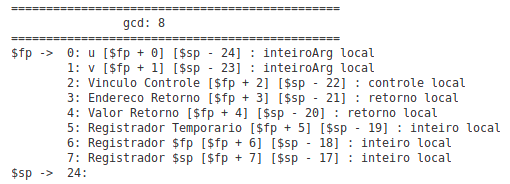
\includegraphics[scale=0.6]{imgs/Codigo/Saida_Memoria.png}
\legend{Fonte: O Autor }
\end{figure}

\begin{figure}[tbhp]
\centering 
\caption{Estrutura de dados para armazenar e gerenciar a memória da pilha de funções, presente no arquivo \nohyphens{``memoria.h''}} 
\label{fig:StructsMemoria}
\graphicspath{ {./imgs/} } 
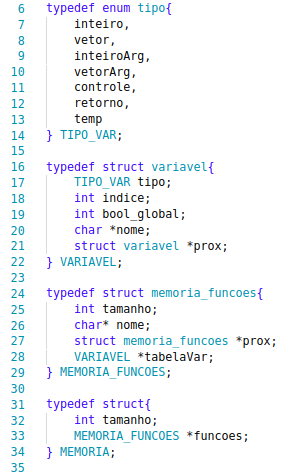
\includegraphics[scale=0.4]{imgs/Codigo/Struct_Memoria.png}
\legend{Fonte: O Autor }
\end{figure}

Outra estrutura que será importante para a geração do código binário é as \emph{labels} e os seus endereços de onde estão no código \emph{assembly}, como ilustrado na \autoref{fig:StructsLabels}. A geração dessa estrutura facilita a busca dos valores dos endereços, já que não é mais preciso percorrer todo o vetor de código \emph{assembly} para encontrar onde ela está localizada.

\begin{figure}[tbhp]
\centering 
\caption{Estrutura de dados para armazenar e gerenciar as \emph{labels} presentes no código \emph{assembly} \nohyphens{``label.h''}} 
\label{fig:StructsLabels}
\graphicspath{ {./imgs/} } 
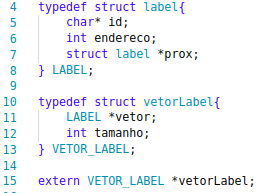
\includegraphics[scale=0.6]{imgs/Codigo/Struct_Labels.png}
\legend{Fonte: O Autor }
\end{figure}

Antes de iniciar a geração do código \emph{assembly} é necessário inicializar a memória com duas pilhas iniciais: 1) ``variáveis globais'', em que todas as variáveis que não estiverem dentro de um escopo de uma função serão adicionadas nessa partição da memória, e 2) parâmetros, já que uma pilha separada na memória deverá ser criada para armazenar as passagens de parâmetros antes da realização de uma chamada de função. 

Após a inicialização do vetor do código, a primeira instrução a ser adicionada deverá ser um jump para a função ``main'', já que a execução do código deve iniciar por ela. Assim, o método ``assembly'', ilustrado na \autoref{fig:CodAssemblyIniciar}, irá percorrer todas as instruções do código intermediário e para cada uma terá uma conversão para o código ``assembly'', que será realizada na função ``geraAssembly''.

\begin{figure}[tbhp]
\centering 
\caption{Função ``assembly'' utilizada para inicializar a geração do código \emph{assembly} para o processador MIPS em \nohyphens{``assembly.c''}} 
\label{fig:CodAssemblyIniciar}
\graphicspath{ {./imgs/} } 
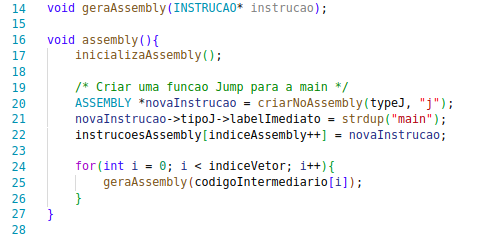
\includegraphics[scale=0.6]{imgs/Codigo/Cod_Assembly.png}
\legend{Fonte: O Autor }
\end{figure}

A função ``geraAssembly'' deve filtrar qual a operação atual daquele código intermediário, para que assim ele possa converter corretamente. A \autoref{fig:CodGerarAssembly} ilustra esse processo para algumas instruções. Para criar uma nova instrução, basta utilizar a função ``criarNoAssembly'', atribuindo como parâmetros os valores do tipo da instrução e o seu nome, que ela irá retornar um ponteiro para uma estrutura ASSEMBLY com o tipo dela inicializada internamente. Dessa forma, basta atribuir os demais valores diretamente a instrução a depender do que deve ser realizado. Essas informações que serão inseridas já são provenientes do código intermediário, como, por exemplo, os valores de quais registradores serão utilizados e quais são as variáveis envolvidas. 

Para a maior parte das instruções de código intermediário basta adicionar apenas uma única instrução para a máquina MIPS e, portanto, são mais diretas de serem interpretadas. Instruções que demandam passos diferentes serão explicadas em suas devidas seções a seguir. 

\begin{figure}[H]
\centering 
\caption{Função ``geraAssembly'' utilizada para gerar efetivamente o código \emph{assembly} para o processador MIPS, presente no arquivo \nohyphens{``assembly.c''}} 
\label{fig:CodGerarAssembly}
\graphicspath{ {./imgs/} } 
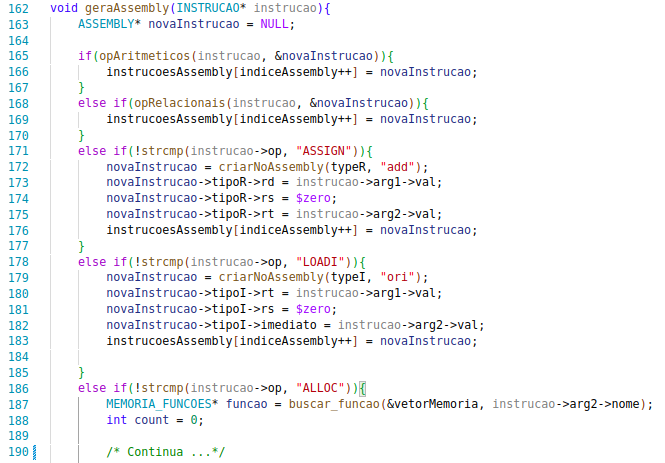
\includegraphics[scale=0.6]{imgs/Codigo/Cod_GeraAssembly.png}
\legend{Fonte: O Autor }
\end{figure}

\subsubsection{Variáveis Inteiras e Vetores}

Para realizar a alocação de memória das variáveis existem duas instruções distintas de código intermediário: ``ALLOC'' e ``ARG''. A primeira é responsável por separar um espaço na memória para variáveis estáticas declaradas internamente naquele escopo, seja da função atual ou global (\autoref{fig:AssemblyALLOC}). Já a segunda é responsável por separar um espaço para as variáveis que foram adicionadas com parâmetro na chamada daquela função (\autoref{fig:AssemblyARG}). 

É possível verificar pelas duas figuras que são utilizadas duas funções: 1) \nohyphens{``buscar\_funcao''} realiza uma busca na estrutura da memória para encontrar a função desejada e 2) ``insere\_variavel'' para inserir a nova variável no espaço livre da função encontrada anteriormente. Para a alocação de vetores, basta adicionar a quantidade de índices passada na declaração do mesmo. Note que nenhuma instrução do código \emph{assembly} foi gerada por enquanto, apenas as configurações internas do compilador.

\begin{figure}[htbp]
\centering 
\caption{Verificação para a instrução ALLOC presente em \nohyphens{``assembly.c''}} 
\label{fig:AssemblyALLOC}
\graphicspath{ {./imgs/} } 
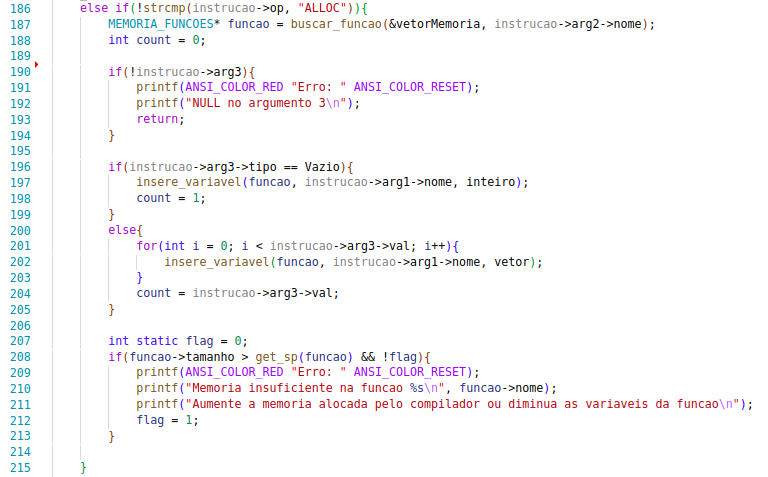
\includegraphics[scale=0.5]{imgs/Codigo/Assembly_ALLOC.png}
\legend{Fonte: O Autor }
\end{figure}


\begin{figure}[htbp]
\centering 
\caption{Verificação para a instrução ARG presente em \nohyphens{``assembly.c''}} 
\label{fig:AssemblyARG}
\graphicspath{ {./imgs/} } 
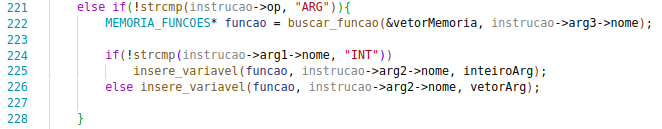
\includegraphics[scale=0.5]{imgs/Codigo/Assembly_ARG.png}
\legend{Fonte: O Autor }
\end{figure}

Para utilizar as variáveis presentes nessas memórias, é preciso recorrer as instruções de acesso a memória, seja de escrita ou leitura. A explicação a seguir será apenas para as instruções de ``LOAD'', mas as instruções de ``STORE'' é um caso análogo a esse.

Para a realização de uma leitura a um valor inteiro basta utilizar o ponteiro \$fp como valor de referência e avançar o valor inteiro em relação a ele, por meio da função ``get\_fp\_relation''. Por meio do exemplo da \autoref{fig:SaidaMemoria}, caso queira ser acessado o valor da variável ``v'', basta passar como registrador base o valor de \$fp e incrementar 1. A implementação pode ser visualizada na \autoref{fig:AssemblyLOAD2} no último \emph{else}.

\begin{figure}[htbp]
\centering 
\caption{Verificação para a instrução LOAD para vetores alocados no escopo da função, presente em \nohyphens{``assembly.c''}} 
\label{fig:AssemblyLOAD1}
\graphicspath{ {./imgs/} } 
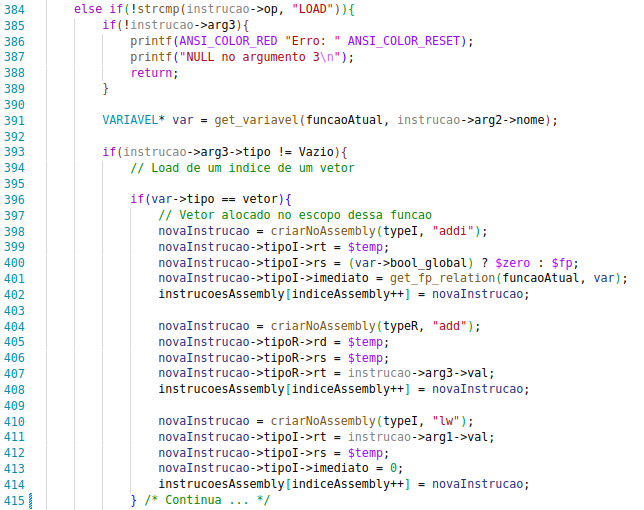
\includegraphics[scale=0.5]{imgs/Codigo/Assembly_LOAD_Vetor.png}
\legend{Fonte: O Autor }
\end{figure}

\begin{figure}[htbp]
\centering 
\caption{Verificação para a instrução LOAD para vetores passados como argumento e variáveis inteiras, presente em \nohyphens{``assembly.c''}} 
\label{fig:AssemblyLOAD2}
\graphicspath{ {./imgs/} } 
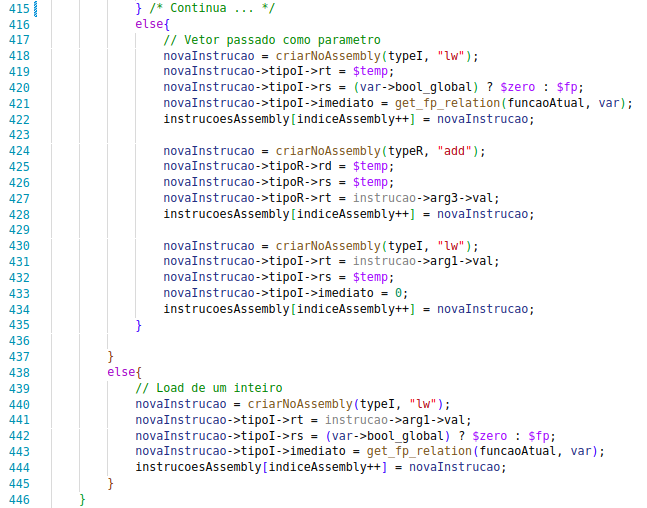
\includegraphics[scale=0.5]{imgs/Codigo/Assembly_LOAD_Inteiros.png}
\legend{Fonte: O Autor }
\end{figure}

Para o caso da variável ser um vetor, é preciso modificar a lógica utilizada para acessá-lo. Obtemos da instrução intermediário ``LOAD'' o valor do índice a ser acessado dentro de um registrador, contudo como o processador implementado apenas suporta utilizar como deslocamento da instrução ``lw'' um valor imediato, é preciso, primeiramente, realizar uma soma entre o valor desse índice a ser acessado com o valor do ponteiro \$fp. Isso é realizado na implementação na \autoref{fig:AssemblyLOAD1} nas instruções ``addi'' e ``add''. Por fim, como o valor atual do registrador \$temp é o endereço exato da memória daquele índice do vetor, basta realizar um ``lw'' com o valor imediato igual a zero.

Dessa forma, para vetores passados como argumento existe apenas uma única modificação que é a necessidade de realizar um ``lw'' no ponteiro armazenado na área de parâmetros da função, que aponta diretamente para o início do vetor na outra função que o alocou. Isso está ilustrado na \autoref{fig:AssemblyLOAD2} no primeiro \emph{else}.


Por fim, para o caso de variáveis globais, basta trocar o valor do ponteiro \$fp pelo registrador \$zero, já que todos as variáveis globais são armazenadas no início da memória de dados.

\subsubsection{Chamada de Funções}

Existem cinco instruções importantes para que seja possível realizar a chamada de uma função, sendo elas: ``FUN'', ``END'', ``PARAM'', ``CALL'' e ``RET''. Elas serão explicadas separadamente, em conjunto com do código gerado em \emph{assembly}.

Para adicionar um valor como parâmetro primeiro é preciso verificar qual o tipo da variável, já que caso ela seja um vetor terá algumas peculiaridades que devem ser levadas em consideração. Ao ser encontrada uma instrução ``PARAM'' (\autoref{fig:AssemblyPARAM}), considerando uma variável inteira, basta adicionar o seu valor na pilha de parâmetros, por meio do registrador \$pilha. Caso seja um vetor, não é o valor que será passado como argumento, mas sim o ponteiro para o início dos seus valores, dessa forma caso ele tenha sido declarado dentro do escopo da função atual (ou seja global), primeiro é preciso somar o valor do ponteiro de referência desejado (\$fp ou \$zero) com a sua relação entre eles e, assim, basta salvar esse valor na pilha. Caso esse vetor já seja um vetor argumento - passado por uma outra função - basta recuperar e salvar na pilha o valor desse ponteiro.

\begin{figure}[H]
\centering 
\caption{Verificação para a instrução PARAM, presente em \nohyphens{``assembly.c''}} 
\label{fig:AssemblyPARAM}
\graphicspath{ {./imgs/} } 
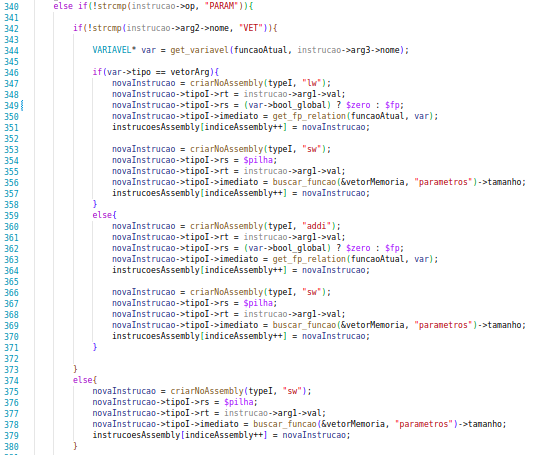
\includegraphics[scale=0.5]{imgs/Codigo/Assembly_Param.png}
\legend{Fonte: O Autor }
\end{figure}

Ao realizar uma chamada de função `CALL'' primeiro é preciso realizar a retirada da pilha de parâmetros para poder armazená-los no ínício da moldura da próxima função, ou seja, no valor do \$sp + k, em que k é o valor atual do parâmetro a ser salvo (primeiro parâmetro é k igual a 1, segundo é k igual a 2 e assim por diante). 

Após realizado esse procedimento dos parâmetros, é preciso salvar o valor de controle da função atual na moldura da próxima, no campo de ``vinculo de controle''. Dessa forma, a próxima função poderá acessar sempre que necessário a função que a chamou.

Como os valores de início e fim da moldura serão distintos nessa nova função, também é necessário alterar os valor de \$fp e \$sp para ficarem condizentes. Dessa forma, como as molduras são padronizadas em 25 índices, basta somar esse valor em cada um dos ponteiros. 

Por fim, para ir até o inicio do código de máquina da próxima função, basta realizar um \emph{jump and link} (jal), que é a função responsável em desviar para a \emph{label} da nova função e salvar o endereço de retorno para a função que a chamou em um registrador específico \$ra. Esse endereço de retorno é importante já que quando a função for realizar um retorno ela precisa saber exatamente para onde ela precisa voltar para continuar com o andamento do código.

Cabe ressaltar que existem dois tipos de funções que podem ser chamadas, porém não precisam estar declaradas internamente no código de programação do usuário: ``output'' e ``input''. Cada uma delas possuem instruções binárias específicas e com funcionalidades já programadas pelo processador em questão. Dessa forma, basta converter as chamadas dessas funções em suas respectivas instruções \emph{assembly} ``out'' e ``in'', realizando a passagem dos parâmetros desejados, advindos do código intermediário. 

As Figuras \ref{fig:AssemblyCALL1}, \ref{fig:AssemblyCALL2} e \ref{fig:AssemblyCALL3} ilustram o código para a conversão do código intermediário para \emph{assembly} para o ``CALL'' explicado anteriormente.

\begin{figure}[H]
\centering 
\caption{Geração de código \emph{assembly} para a instrução intermediária CALL - parte 1 - presente no arquivo ``assembly.c''} \label{fig:AssemblyCALL1}
\graphicspath{ {./imgs/} } 
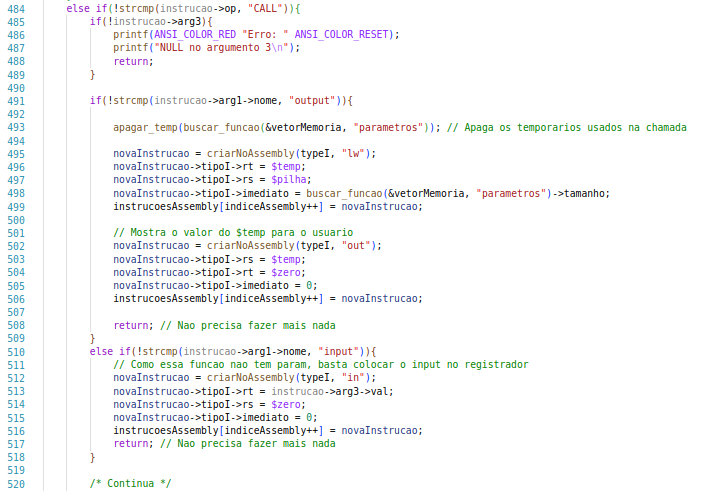
\includegraphics[scale=0.4]{imgs/Codigo/Cod_Assembly_Call1.png}
\legend{Fonte: O Autor }
\end{figure}

\begin{figure}[H]
\centering 
\caption{Geração de código \emph{assembly} para a instrução intermediária CALL - parte 2 - presente no arquivo ``assembly.c''} \label{fig:AssemblyCALL2}
\graphicspath{ {./imgs/} } 
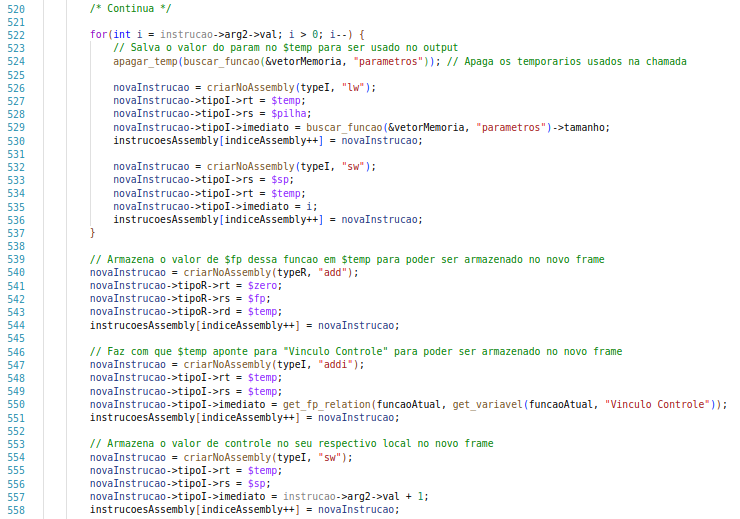
\includegraphics[scale=0.4]{imgs/Codigo/Cod_Assembly_Call2.png}
\legend{Fonte: O Autor }
\end{figure}

\begin{figure}[H]
\centering 
\caption{Geração de código \emph{assembly} para a instrução intermediária CALL - parte 3 - presente no arquivo ``assembly.c''} \label{fig:AssemblyCALL3}
\graphicspath{ {./imgs/} } 
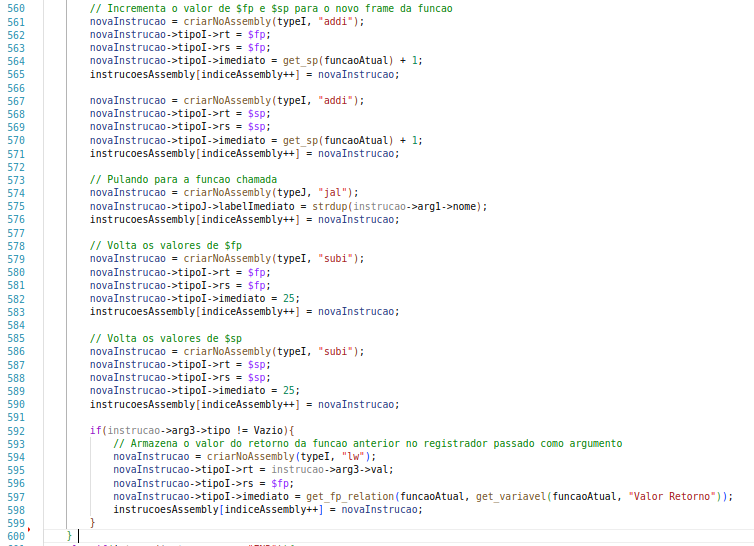
\includegraphics[scale=0.4]{imgs/Codigo/Cod_Assembly_Call3.png}
\legend{Fonte: O Autor }
\end{figure}


No momento que a função que foi chamada for finalizada ela irá voltar na instrução seguinte ao ``jal''. Como a função foi alterada novamente, os valores dos ponteiros devem voltar ao que eram antes. Nesse caso, basta subtrair o valor 25. Para finalizar o procedimento, caso a função tenha retornado algo, basta realizar uma leitura na área da memória ``valor de retorno''. O motivo de realizar esse procedimento será explicado adiante, durante a função ``RET''.

A instrução de código intermediário ``FUN'' tem a fundamental importância de sinalizar o inicio de uma nova função no código digitado pelo usuário. Ao convertê-la para o código \emph{assembly}, basta realizar uma única ação, que é armazenar o valor presente no registrador \$ra dentro do seu \emph{frame}, no campo ``Valor de Retorno''. Assim, quando o procedimento seja finalizado, uma instrução de \emph{jump} incondicional será realizada para quem a chamou. Caso a função seja a ``main'', alguns procedimento a mais terão que ser realizados: 1) Inicializar os valores de \$fp e \$sp considerando os valores das variáveis globais já separadas na memória; e 2) inicializar o registrador \$pilha para o valor fixo para a pilha de parâmetros. A \autoref{fig:AssemblyFUN} representa o código para a verificação anterior.

\begin{figure}[H]
\centering 
\caption{Geração de código \emph{assembly} para a instrução intermediária FUN, presente no arquivo ``assembly.c''} \label{fig:AssemblyFUN}
\graphicspath{ {./imgs/} } 
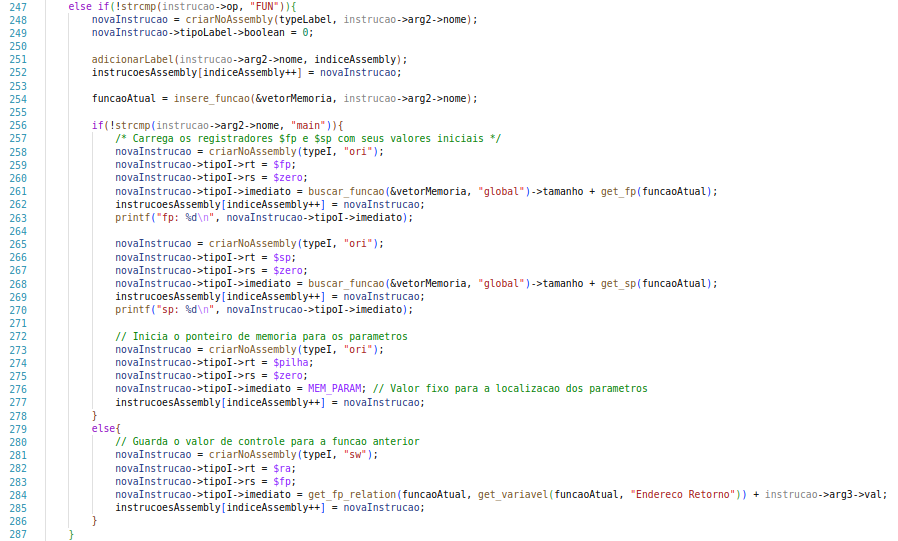
\includegraphics[scale=0.4]{imgs/Codigo/Cod_Assembly_Fun.png}
\legend{Fonte: O Autor }
\end{figure}


Por fim, basta exemplificar o que será feito nas instruções de ``RET'' (\autoref{fig:AssemblyRET}) e ``END'' (\autoref{fig:AssemblyEnd}), já que suas funcionalidades estão interligadas. Na primeira, será preciso retornar um valor para a função anterior na pilha da memória, já que ela está aguardando esse valor para continuar a sua rotina, dessa forma foi programado para que todos os resultados a serem retornados devem ser armazenados no campo ``valor de retorno'', como citado anteriormente. Dessa forma, basta carregar o valor que aponta para \emph{frame} anterior e armazenar o valor indicado no registrador. Já a segunda instrução, basta ler da memória o endereço de retorno, aramzená-lo em um registrador e, por fim, realizar um \emph{jump register}. Caso a instrução de finalização seja da função ``main'', nada será feito, já que o programa será finalizado na instrução ``HALT'' seguinte.

\begin{figure}[H]
\centering 
\caption{Geração de código \emph{assembly} para a instrução intermediária END presente no arquivo ``assembly.c''} \label{fig:AssemblyEnd}
\graphicspath{ {./imgs/} } 
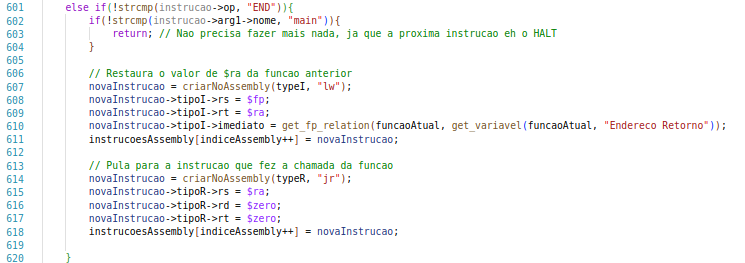
\includegraphics[scale=0.4]{imgs/Codigo/Cod_Assembly_End.png}
\legend{Fonte: O Autor }
\end{figure}

\begin{figure}[H]
\centering 
\caption{Geração de código \emph{assembly} para a instrução intermediária RET presente no arquivo ``assembly.c''} \label{fig:AssemblyRET}
\graphicspath{ {./imgs/} } 
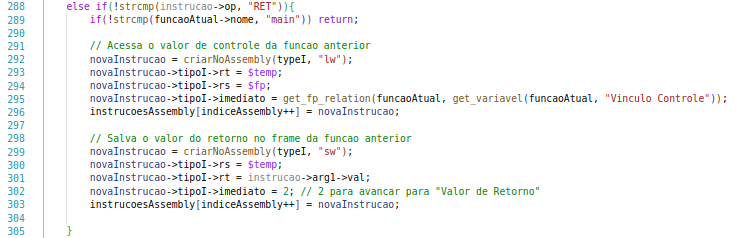
\includegraphics[scale=0.4]{imgs/Codigo/Cod_Assembly_Ret.png}
\legend{Fonte: O Autor }
\end{figure}

\subsection{Código Binário}

Após obter o código \emph{assembly}, basta convertê-lo para o valor binário correspondente para cada campo designado. Por ser apenas um processo direto de conversão um para um ele não possuí muitas complicações de implementação no projeto do compilador. A \autoref{fig:StructsBinario} ilustra as estruturas para armazenar os valores binários antes de realizar a conversão para um arquivo externo.

\begin{figure}[htbp]
\centering 
\caption{Estruturas para armazenar os valores binários do código, presente no arquivo \nohyphens{``binario.h''}} 
\label{fig:StructsBinario}
\graphicspath{ {./imgs/} } 
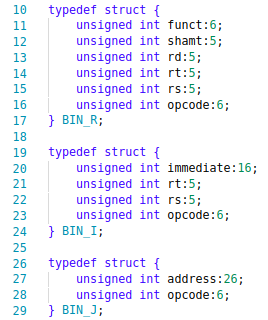
\includegraphics[scale=0.6]{imgs/Codigo/Struct_CodigoBinario.png}
\legend{Fonte: O Autor }
\end{figure}

A estrutura foi implementada seguindo o padrão já mencionado das instruções nas Tabelas \ref{tab:FormatInstrTypeR}, \ref{tab:FormatInstrTypeI} e \ref{tab:FormatInstrTypeJ}. Os dois pontos após a declaração das variáveis representam a quantidade de bits que serão utilizados para armazenar os valores para aquele campo em específico e, dessa forma, a soma dos bits utilizados deve ser igual a 32, o equivalente ao tamanho de um ``unsigned int''. Com isso, todas as \emph{structs} geradas irão armazenar exatamente 32 bits e não será preciso realizar nenhum tratamento especial para a exclusão de valores a mais de variáveis maiores e, portanto, ao realizar a impressão no arquivo basta mostrar todos os bits armazenados dentro dessa estrutura.

\begin{figure}[htbp]
\centering 
\caption{Funçao ``binario'' utilizada para converter o código \emph{assembly} para binário, implementado no arquivo \nohyphens{``binario.c''}} 
\label{fig:GeracaoBinario}
\graphicspath{ {./imgs/} } 
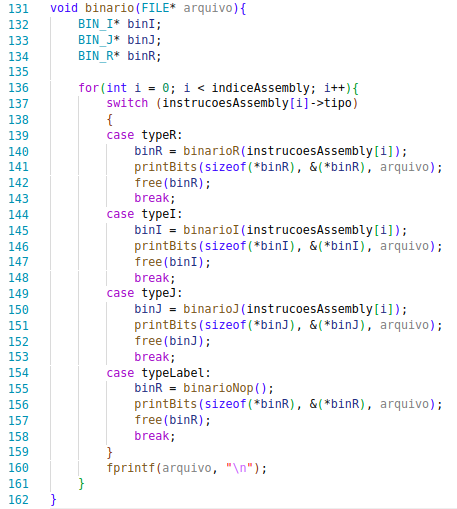
\includegraphics[scale=0.5]{imgs/Codigo/Binario_Geracao.png}
\legend{Fonte: O Autor }
\end{figure}

Na \autoref{fig:GeracaoBinario} a função ``binario'' irá realizar um laço para percorrer todas as instruções \emph{assembly}, separando elas por tipo e enviando para métodos específicos para tratar cada uma delas, representados pela \autoref{fig:ConversaoBinario}. As funções ``get\_opcode'' e ``get\_funct'', ilustradas na \autoref{fig:BinarioOpcodeFunct}, tem o propósito de retornar o \emph{opcode} e o \emph{funct} das instruções, com base no código binário descrito nas Tabelas \ref{tab:FormatInstrTypeR}, \ref{tab:FormatInstrTypeI} e \ref{tab:FormatInstrTypeJ}. Já as demais funções apenas retornam o mesmo valor passado como parâmetro, já que os valores de endereços, registradores e imediatos não precisam de conversão.

\begin{figure}[htbp]
\centering 
\caption{Funções específicas para a conversão do código \emph{assembly} em formatos do tipo R, I e J, respectivamente. Implementado no arquivo \nohyphens{``binario.c''}} 
\label{fig:ConversaoBinario}
\graphicspath{ {./imgs/} } 
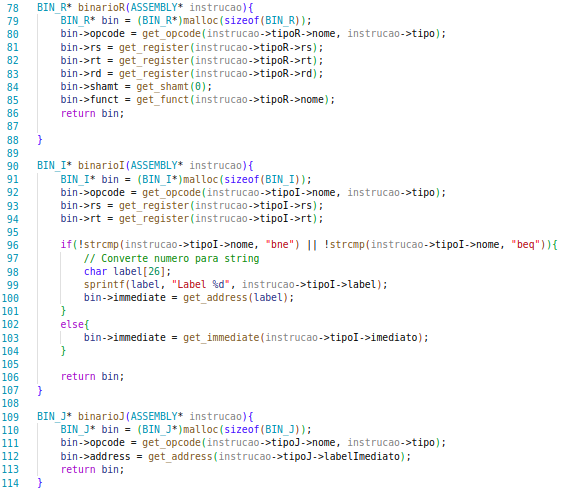
\includegraphics[scale=0.5]{imgs/Codigo/Binario_Conversao.png}
\legend{Fonte: O Autor }
\end{figure}

\begin{figure}[htbp]
\centering 
\caption{Funções para conversão do nome da instrução em seu opcode e funct (para tipo R) em binário. Presente no arquivo \nohyphens{``binario.c''}} 
\label{fig:BinarioOpcodeFunct}
\graphicspath{ {./imgs/} } 
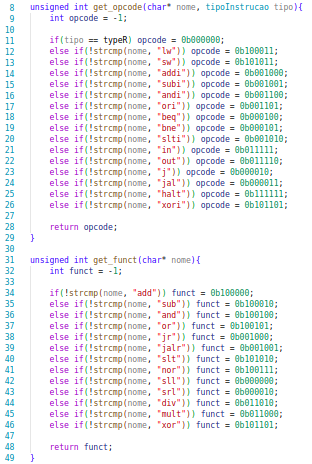
\includegraphics[scale=0.5]{imgs/Codigo/Binario_opcode_funct.png}
\legend{Fonte: O Autor }
\end{figure}


Por fim, para imprimir o valor do código binário em um arquivo, a função ``printBits'' foi implementada (\autoref{fig:BinarioPrintBits}) para receber o endereço de uma estrutura qualquer em conjunto com o seu tamanho e, assim, acessar os seus valores armazenados, mostrando bit a bit em um arquivo externo, que também é passado como argumento. 

\begin{figure}[htbp]
\centering 
\caption{Função para mostrar o valor binário para um arquivo esterno. Presente no arquivo \nohyphens{``binario.c''}} 
\label{fig:BinarioPrintBits}
\graphicspath{ {./imgs/} } 
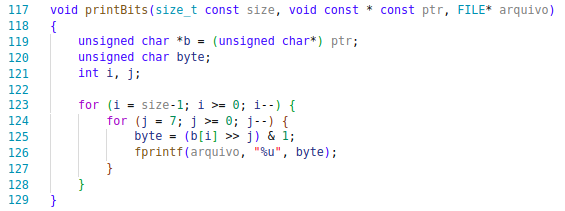
\includegraphics[scale=0.5]{imgs/Codigo/Binario_printbits.png}
\legend{Fonte: O Autor }
\end{figure}

\chapter{Resultados}
Para demonstrar o funcionamento do compilador, três exemplos serão testados e com os resultados obtidos de cada uma das três etapas da fase de geração de código fonte.

\section{Fatorial Recursivo}

\subsection{Código Fonte}
\begin{lstlisting} [language=C]
int fatorial(int n){
    int vfat; 

    if (n == 1){
        return (1);
    }
    else{
        vfat = fatorial(n-1)*n;
        return (vfat);
    }
}

int main(void){
  int x;
  x = input();

  output(fatorial(x));

  return 0;
}

\end{lstlisting}



\subsection{Relação entre Códigos}

Após adicionar o arquivo do código fonte como entrada no compilador finalizado, os resultados para o código intermediário, \emph{assembly} e binário pode ser observado na \autoref{tab:ResultadosFatorial}.

% \usepackage{tabularray}
\begin{longtblr}[
  caption = {Geração de códigos da fase de síntese para o programa fatorial recursivo},
  label = {tab:ResultadosFatorial},
]{
  row{1} = {c},
  cell{3}{1} = {r=2}{},
  cell{5}{2} = {c},
  cell{5}{3} = {c},
  cell{7}{2} = {c},
  cell{7}{3} = {c},
  cell{10}{1} = {r=3}{},
  cell{15}{1} = {r=2}{},
  cell{25}{1} = {r=11}{},
  cell{41}{1} = {r=2}{},
  cell{46}{1} = {r=2}{},
  cell{48}{1} = {r=4}{},
  cell{52}{2} = {c},
  cell{52}{3} = {c},
  cell{59}{1} = {r=11}{},
  cell{71}{1} = {r=2}{},
  cell{73}{2} = {c},
  cell{73}{3} = {c},
  cell{76}{2} = {c},
  cell{76}{3} = {c},
  vlines,
  hline{1-3,5-10,13-15,17-25,36-41,43-46,48,52-59,70-71,73-78} = {-}{},
  hline{4,11-12,16,26-35,42,47,49-51,60-69,72} = {2-3}{},
}
Código Intermediário & Código Assembly & Código Binário\\
GOTO, main, -, - & j main & 00001000000000000000000000101100\\
FUN, INT, fatorial, \$t1 & fatorial: & 00000011111111111111100000100000\\
 & sw \$ra 2(\$fp) & 10101111101111100000000000000010\\
ARG, INT, n, fatorial & - & -\\
LOAD, \$t0, n, - & lw \$t0 0(\$fp) & 10001111101000000000000000000000\\
ALLOC, vfat, fatorial, - & - & -\\
LOAD, \$t0, n, - & lw \$t0 0(\$fp) & 10001111101000000000000000000000\\
LOADI, \$t1, 1, - & ori \$t1 \$zero 1 & 00110111111000010000000000000001\\
EQ, \$t0, \$t1, \$t2 & slt \$t2 \$t0 \$t1 & 00000000000000010001000000101010\\
 & slt \$t2 \$t1 \$t0 & 00000000001000000001000000101010\\
 & xori \$t2 \$t2 1 & 10110100010000100000000000000001\\
IFF, \$t2, L1, - & beq \$t2 \$zero Label 1 & 00010011111000100000000000001111\\
LOADI, \$t3, 1, - & ori \$t3 \$zero 1 & 00110111111000110000000000000001\\
RET, \$t3, -, - & lw \$temp 1(\$fp) & 10001111101110110000000000000001\\
 & sw \$t3 2(\$temp) & 10101111011000110000000000000010\\
GOTO, L0, -, - & j Label 0 & 00001000000000000000000000101001\\
GOTO, L2, -, - & j Label 2 & 00001000000000000000000000101000\\
LABEL, L1, -, - & Label 1: & 00000011111111111111100000100000\\
LOAD, \$t4, vfat, - & lw \$t4 7(\$fp) & 10001111101001000000000000000111\\
LOAD, \$t0, n, - & lw \$t0 0(\$fp) & 10001111101000000000000000000000\\
LOADI, \$t5, 1, - & ori \$t5 \$zero 1 & 00110111111001010000000000000001\\
SUB, \$t0, \$t5, \$t6 & sub \$t6 \$t0 \$t5 & 00000000000001010011000000100010\\
PARAM, \$t6, INT, - & sw \$t6 0(\$pilha) & 10101111010001100000000000000000\\
CALL, fatorial, 1, \$t7 & lw \$temp 0(\$pilha) & 10001111010110110000000000000000\\
 & sw \$temp 1(\$sp) & 10101111100110110000000000000001\\
 & add \$temp \$fp \$zero & 00000011101111111101100000100000\\
 & addi \$temp \$temp 1 & 00100011011110110000000000000001\\
 & sw \$temp 2(\$sp) & 10101111100110110000000000000010\\
 & addi \$fp \$fp 25 & 00100011101111010000000000011001\\
 & addi \$sp \$sp 25 & 00100011100111000000000000011001\\
 & jal fatorial & 00001100000000000000000000000001\\
 & subi \$fp \$fp 25 & 00100111101111010000000000011001\\
 & subi \$sp \$sp 25 & 00100111100111000000000000011001\\
 & lw \$t7 3(\$fp) & 10001111101001110000000000000011\\
LOAD, \$t0, n, - & lw \$t0 0(\$fp) & 10001111101000000000000000000000\\
MULT, \$t7, \$t0, \$t8 & mult \$t8 \$t7 \$t0 & 00000000111000000100000000011000\\
ASSIGN, \$t4, \$t8, - & add \$t4 \$zero \$t8 & 00000011111010000010000000100000\\
STORE, vfat, \$t4, - & sw \$t4 7(\$fp) & 10101111101001000000000000000111\\
LOAD, \$t4, vfat, - & lw \$t4 7(\$fp) & 10001111101001000000000000000111\\
RET, \$t4, -, - & lw \$temp 1(\$fp) & 10001111101110110000000000000001\\
 & sw \$t4 2(\$temp) & 10101111011001000000000000000010\\
GOTO, L0, -, - & j Label 0 & 00001000000000000000000000101001\\
LABEL, L2, -, - & Label 2: & 00000011111111111111100000100000\\
LABEL, L0, -, - & Label 0: & 00000011111111111111100000100000\\
END, fatorial, -, - & lw \$ra 2(\$fp) & 10001111101111100000000000000010\\
 & jr \$zero \$ra \$zero & 00000011110111111111100000001000\\
FUN, INT, main, 0 & main: & 00000011111111111111100000100000\\
 & ori \$fp \$zero 0 & 00110111111111010000000000000000\\
 & ori \$sp \$zero 24 & 00110111111111000000000000011000\\
 & ori \$pilha \$zero 1000 & 00110111111110100000001111101000\\
ALLOC, x, main, - & - & -\\
LOAD, \$t9, x, - & lw \$t9 6(\$fp) & 10001111101010010000000000000110\\
CALL, input, 0, \$t10 & in \$t10 \$zero 0 & 01111111111010100000000000000000\\
ASSIGN, \$t9, \$t10, - & add \$t9 \$zero \$t10 & 00000011111010100100100000100000\\
STORE, x, \$t9, - & sw \$t9 6(\$fp) & 10101111101010010000000000000110\\
LOAD, \$t9, x, - & lw \$t9 6(\$fp) & 10001111101010010000000000000110\\
PARAM, \$t9, INT, - & sw \$t9 0(\$pilha) & 10101111010010010000000000000000\\
CALL, fatorial, 1, \$t11 & lw \$temp 0(\$pilha) & 10001111010110110000000000000000\\
 & sw \$temp 1(\$sp) & 10101111100110110000000000000001\\
 & add \$temp \$fp \$zero & 00000011101111111101100000100000\\
 & addi \$temp \$temp 0 & 00100011011110110000000000000000\\
 & sw \$temp 2(\$sp) & 10101111100110110000000000000010\\
 & addi \$fp \$fp 25 & 00100011101111010000000000011001\\
 & addi \$sp \$sp 25 & 00100011100111000000000000011001\\
 & jal fatorial & 00001100000000000000000000000001\\
 & subi \$fp \$fp 25 & 00100111101111010000000000011001\\
 & subi \$sp \$sp 25 & 00100111100111000000000000011001\\
 & lw \$t11 2(\$fp) & 10001111101010110000000000000010\\
PARAM, \$t11, INT, - & sw \$t11 0(\$pilha) & 10101111010010110000000000000000\\
CALL, output, 1, - & lw \$temp 0(\$pilha) & 10001111010110110000000000000000\\
 & out \$zero \$temp 0 & 01111011011111110000000000000000\\
RET, \$t31, -, - & - & -\\
GOTO, L3, -, - & j Label 3 & 00001000000000000000000001000101\\
LABEL, L3, -, - & Label 3: & 00000011111111111111100000100000\\
END, main, -, - & - & -\\
HALT, -, -, - & halt \$zero & 11111111111111111111111111111111
\end{longtblr}

\legend{Fonte: O Autor }

\subsection{Teste FPGA}

Para finalizar, um teste foi realizada com o envio do processador programado para operar o programa anteriormente compilado. O valor de entrada do usuário será de 6, portanto o valor resultante deverá ser 720.

\begin{figure}[H]
\centering 
\caption{Inserindo o valor decimal 6 para o cálculo do fatorial na placa FPGA} 
\label{fig:FPGAFatorialEntrada}
\graphicspath{ {./imgs/} } 
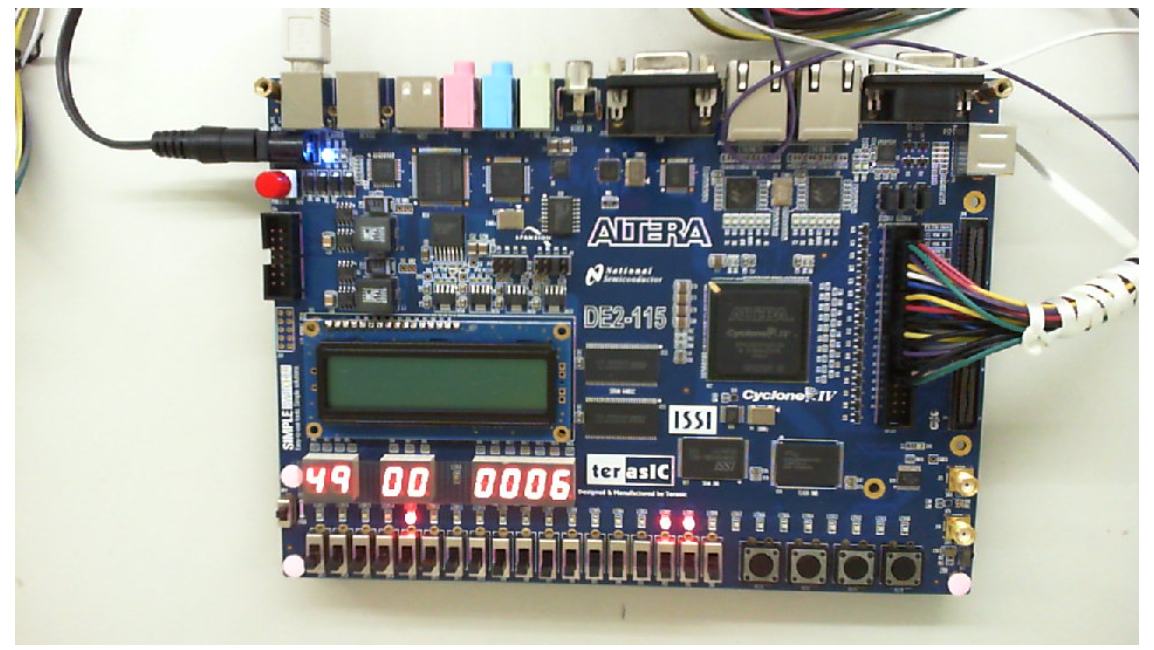
\includegraphics[scale=0.43]{imgs/Resultados/Fatorial_FPGA_Entrada.png}
\legend{Fonte: O Autor }
\end{figure}

\begin{figure}[H]
\centering 
\caption{Resultado obtido para o cálculo do fatorial de 6 na placa FPGA} 
\label{fig:FPGAFatorialSaida}
\graphicspath{ {./imgs/} } 
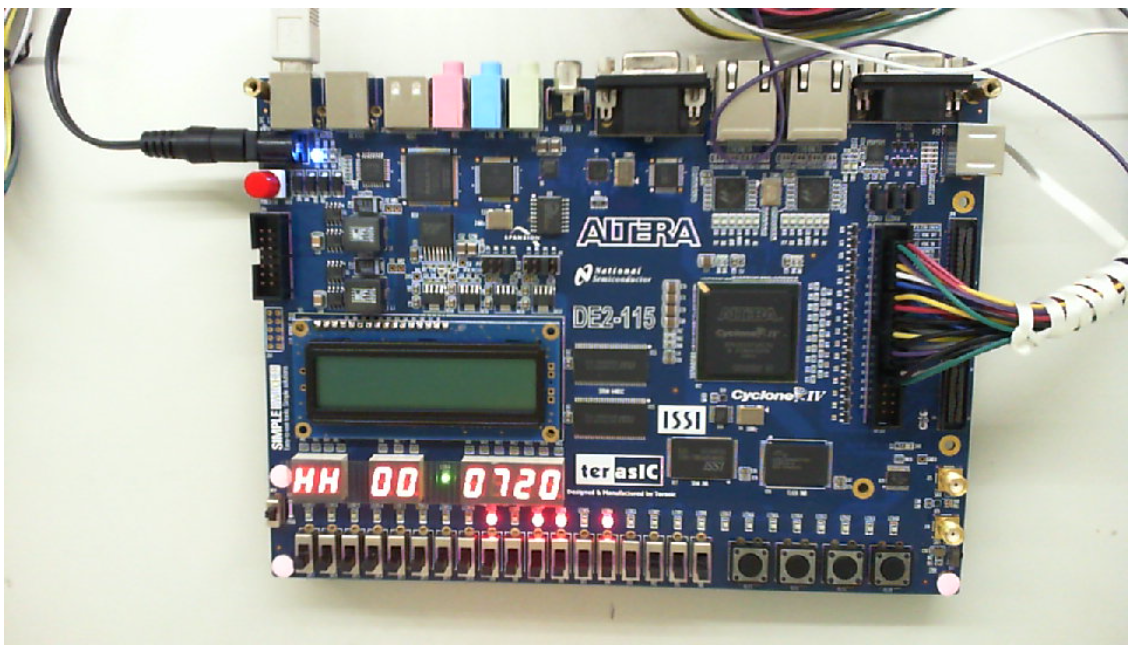
\includegraphics[scale=0.43]{imgs/Resultados/Fatorial_FPGA_Saida.png}
\legend{Fonte: O Autor }
\end{figure}

Considerando os testes realizados nas Figuras \ref{fig:FPGAFatorialEntrada} e \ref{fig:FPGAFatorialSaida}, é constatado que o programa está calculando corretamente o fatorial do número 6, já que o valor corresponde é 720.

\section{Máximo Denominador Comum}

\subsection{Código Fonte}
\begin{lstlisting} [language=C]
int gcd (int u, int v){ 	
    if (v == 0) {return u;}
    else return gcd(v,u-u/v*v);
}

void main(void){	
    int x; int y;

    x = input(); y = input();
    output(gcd(x,y));
}
\end{lstlisting}

\subsection{Relação entre Códigos}

% \usepackage{color}
% \usepackage{rotating}
% \usepackage{tabularray}
% \usepackage{color}
% \usepackage{rotating}
% \usepackage{tabularray}
% \usepackage{color}
% \usepackage{rotating}
% \usepackage{tabularray}
% \usepackage{color}
% \usepackage{rotating}
% \usepackage{tabularray}
\begin{longtblr}[
  caption = {Resultado da geração de códigos para o programa máximo denominador comum},
  label = {tab:ResultadosMDC},
]{
  row{even} = {t},
  row{1} = {t},
  row{3} = {t},
  row{5} = {t},
  row{7} = {t},
  row{9} = {t},
  row{11} = {t},
  row{13} = {t},
  row{15} = {t},
  row{17} = {t},
  row{19} = {t},
  row{21} = {t},
  row{23} = {t},
  row{25} = {t},
  row{27} = {t},
  row{29} = {t},
  row{31} = {t},
  row{33} = {t},
  row{35} = {t},
  row{37} = {t},
  row{39} = {t},
  row{41} = {t},
  row{43} = {t},
  row{45} = {t},
  row{47} = {t},
  row{49} = {t},
  row{53} = {t},
  row{55} = {t},
  row{57} = {t},
  row{59} = {t},
  row{61} = {t},
  row{63} = {t},
  row{65} = {t},
  row{67} = {t},
  row{69} = {t},
  row{71} = {t},
  row{73} = {t},
  row{75} = {t},
  row{77} = {t},
  row{79} = {t},
  row{81} = {t},
  row{83} = {t},
  row{85} = {t},
  cell{3}{1} = {r=2}{},
  cell{5}{2} = {c},
  cell{5}{3} = {c},
  cell{6}{2} = {c},
  cell{6}{3} = {c},
  cell{10}{1} = {r=3}{},
  cell{15}{1} = {r=2}{},
  cell{30}{1} = {r=13}{},
  cell{43}{1} = {r=2}{},
  cell{48}{1} = {r=2}{},
  cell{51}{1} = {r=3}{},
  cell{51}{2} = {t},
  cell{51}{3} = {t},
  cell{54}{2} = {c},
  cell{54}{3} = {c},
  cell{55}{2} = {c},
  cell{55}{3} = {c},
  cell{68}{1} = {r=13}{},
  cell{82}{1} = {r=2}{},
  cell{85}{2} = {c},
  cell{85}{3} = {c},
  vlines,
  hline{1-3,5-10,13-15,17-30,43,45-48,50,54-68,81-82,84-87} = {-}{},
  hline{4,11-12,16,31-42,44,49,51-53,69-80,83} = {2-3}{},
}
Código Intermediário & Código Assembly & Código Binário\\
GOTO, main, -, - & j main & 00001000000000000000000000101110\\
FUN, INT, gcd, 2 & gcd: & 00000011111111111111100000100000\\
 & sw \$ra 3(\$fp) & 10101111101111100000000000000011\\
ARG, INT, u, gcd & - & -\\
ARG, INT, v, gcd & - & -\\
LOAD, \$t0, u, - & lw \$t0 0(\$fp) & 10001111101000000000000000000000\\
LOAD, \$t1, v, - & lw \$t1 1(\$fp) & 10001111101000010000000000000001\\
LOAD, \$t1, v, - & lw \$t1 1(\$fp) & 10001111101000010000000000000001\\
EQ, \$t1, \$t31, \$t2 & slt \$t2 \$t1 \$zero & 00000000001111110001000000101010\\
 & slt \$t2 \$zero \$t1 & 00000011111000010001000000101010\\
 & xori \$t2 \$t2 1 & 10110100010000100000000000000001\\
IFF, \$t2, L1, - & beq \$t2 \$zero Label 1 & 00010011111000100000000000001111\\
LOAD, \$t0, u, - & lw \$t0 0(\$fp) & 10001111101000000000000000000000\\
RET, \$t0, -, - & lw \$temp 2(\$fp) & 10001111101110110000000000000010\\
 & sw \$t0 2(\$temp) & 10101111011000000000000000000010\\
GOTO, L0, -, - & j Label 0 & 00001000000000000000000000101011\\
GOTO, L2, -, - & j Label 2 & 00001000000000000000000000101010\\
LABEL, L1, -, - & Label 1: & 00000011111111111111100000100000\\
LOAD, \$t1, v, - & lw \$t1 1(\$fp) & 10001111101000010000000000000001\\
PARAM, \$t1, INT, - & sw \$t1 0(\$pilha) & 10101111010000010000000000000000\\
LOAD, \$t0, u, - & lw \$t0 0(\$fp) & 10001111101000000000000000000000\\
LOAD, \$t0, u, - & lw \$t0 0(\$fp) & 10001111101000000000000000000000\\
LOAD, \$t1, v, - & lw \$t1 1(\$fp) & 10001111101000010000000000000001\\
DIV, \$t0, \$t1, \$t3 & div \$t3 \$t0 \$t1 & 00000000000000010001100000011010\\
LOAD, \$t1, v, - & lw \$t1 1(\$fp) & 10001111101000010000000000000001\\
MULT, \$t3, \$t1, \$t4 & mult \$t4 \$t3 \$t1 & 00000000011000010010000000011000\\
SUB, \$t0, \$t4, \$t5 & sub \$t5 \$t0 \$t4 & 00000000000001000010100000100010\\
PARAM, \$t5, INT, - & sw \$t5 1(\$pilha) & 10101111010001010000000000000001\\
CALL, gcd, 2, \$t6 & lw \$temp 1(\$pilha) & 10001111010110110000000000000001\\
 & sw \$temp 2(\$sp) & 10101111100110110000000000000010\\
 & lw \$temp 0(\$pilha) & 10001111010110110000000000000000\\
 & sw \$temp 1(\$sp) & 10101111100110110000000000000001\\
 & add \$temp \$fp \$zero & 00000011101111111101100000100000\\
 & addi \$temp \$temp 2 & 00100011011110110000000000000010\\
 & sw \$temp 3(\$sp) & 10101111100110110000000000000011\\
 & addi \$fp \$fp 25 & 00100011101111010000000000011001\\
 & addi \$sp \$sp 25 & 00100011100111000000000000011001\\
 & jal gcd & 00001100000000000000000000000001\\
 & subi \$fp \$fp 25 & 00100111101111010000000000011001\\
 & subi \$sp \$sp 25 & 00100111100111000000000000011001\\
 & lw \$t6 4(\$fp) & 10001111101001100000000000000100\\
RET, \$t6, -, - & lw \$temp 2(\$fp) & 10001111101110110000000000000010\\
 & sw \$t6 2(\$temp) & 10101111011001100000000000000010\\
GOTO, L0, -, - & j Label 0 & 00001000000000000000000000101011\\
LABEL, L2, -, - & Label 2: & 00000011111111111111100000100000\\
LABEL, L0, -, - & Label 0: & 00000011111111111111100000100000\\
END, gcd, -, - & lw \$ra 3(\$fp) & 10001111101111100000000000000011\\
 & jr \$zero \$ra \$zero & 00000011110111111111100000001000\\
FUN, VOID, main, 0 & main: & 00000011111111111111100000100000\\
 & ori \$fp \$zero 0 & 00110111111111010000000000000000\\
 & ori \$sp \$zero 24 & 00110111111111000000000000011000\\
 & ori \$pilha \$zero 1000 & 00110111111110100000001111101000\\
ALLOC, x, main, - & - & -\\
ALLOC, y, main, - & - & -\\
LOAD, \$t7, x, - & lw \$t7 6(\$fp) & 10001111101001110000000000000110\\
CALL, input, 0, \$t8 & in \$t8 \$zero 0 & 01111111111010000000000000000000\\
ASSIGN, \$t7, \$t8, - & add \$t7 \$zero \$t8 & 00000011111010000011100000100000\\
STORE, x, \$t7, - & sw \$t7 6(\$fp) & 10101111101001110000000000000110\\
LOAD, \$t9, y, - & lw \$t9 7(\$fp) & 10001111101010010000000000000111\\
CALL, input, 0, \$t10 & in \$t10 \$zero 0 & 01111111111010100000000000000000\\
ASSIGN, \$t9, \$t10, - & add \$t9 \$zero \$t10 & 00000011111010100100100000100000\\
STORE, y, \$t9, - & sw \$t9 7(\$fp) & 10101111101010010000000000000111\\
LOAD, \$t7, x, - & lw \$t7 6(\$fp) & 10001111101001110000000000000110\\
PARAM, \$t7, INT, - & sw \$t7 0(\$pilha) & 10101111010001110000000000000000\\
LOAD, \$t9, y, - & lw \$t9 7(\$fp) & 10001111101010010000000000000111\\
PARAM, \$t9, INT, - & sw \$t9 1(\$pilha) & 10101111010010010000000000000001\\
CALL, gcd, 2, \$t11 & lw \$temp 1(\$pilha) & 10001111010110110000000000000001\\
 & sw \$temp 2(\$sp) & 10101111100110110000000000000010\\
 & lw \$temp 0(\$pilha) & 10001111010110110000000000000000\\
 & sw \$temp 1(\$sp) & 10101111100110110000000000000001\\
 & add \$temp \$fp \$zero & 00000011101111111101100000100000\\
 & addi \$temp \$temp 0 & 00100011011110110000000000000000\\
 & sw \$temp 3(\$sp) & 10101111100110110000000000000011\\
 & addi \$fp \$fp 25 & 00100011101111010000000000011001\\
 & addi \$sp \$sp 25 & 00100011100111000000000000011001\\
 & jal gcd & 00001100000000000000000000000001\\
 & subi \$fp \$fp 25 & 00100111101111010000000000011001\\
 & subi \$sp \$sp 25 & 00100111100111000000000000011001\\
 & lw \$t11 2(\$fp) & 10001111101010110000000000000010\\
PARAM, \$t11, INT, - & sw \$t11 0(\$pilha) & 10101111010010110000000000000000\\
CALL, output, 1, - & lw \$temp 0(\$pilha) & 10001111010110110000000000000000\\
 & out \$zero \$temp 0 & 01111011011111110000000000000000\\
LABEL, L3, -, - & Label 3: & 00000011111111111111100000100000\\
END, main, -, - & - & -\\
HALT, -, -, - & halt \$zero & 11111111111111111111111111111111
\end{longtblr}
\legend{Fonte: O Autor }

\subsection{Teste FPGA}

\begin{figure}[H]
\centering 
\caption{Inserindo como primeiro valor o número 15 para o programa do máximo divisor comum} 
\label{fig:FPGAMDCEntrada1}
\graphicspath{ {./imgs/} } 
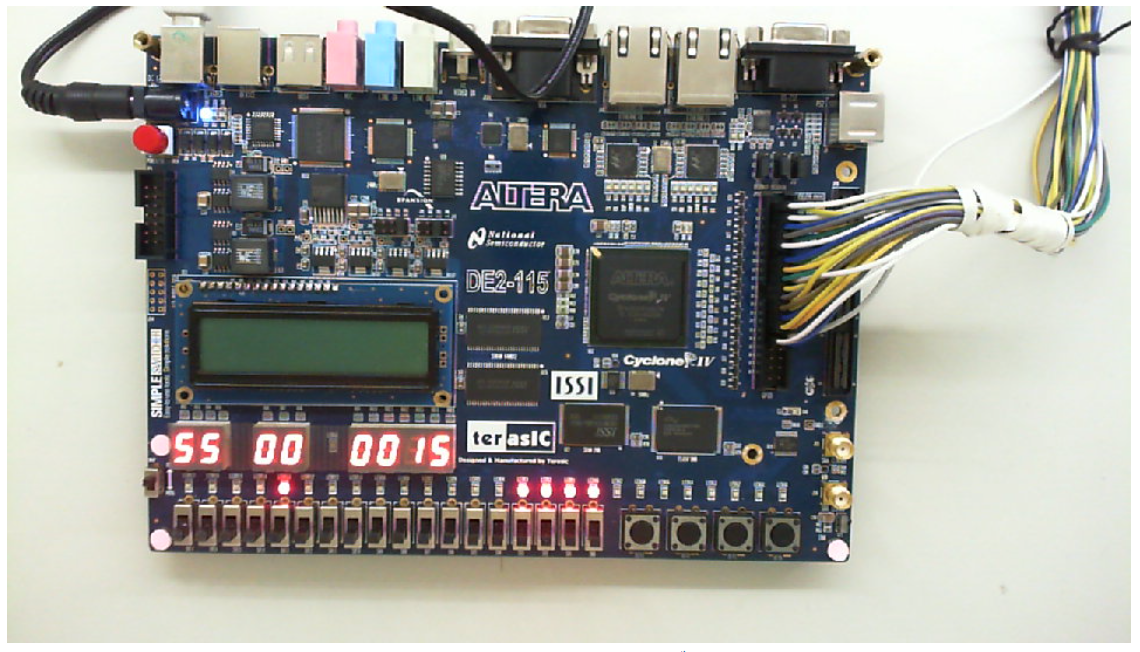
\includegraphics[scale=0.4]{imgs/Resultados/MDC_FPGA_Entrada2.png}
\legend{Fonte: O Autor }
\end{figure}

\begin{figure}[H]
\centering 
\caption{Inserindo como segundo valor o número 20 para o programa do máximo divisor comum} 
\label{fig:FPGAMDCEntrada2}
\graphicspath{ {./imgs/} } 
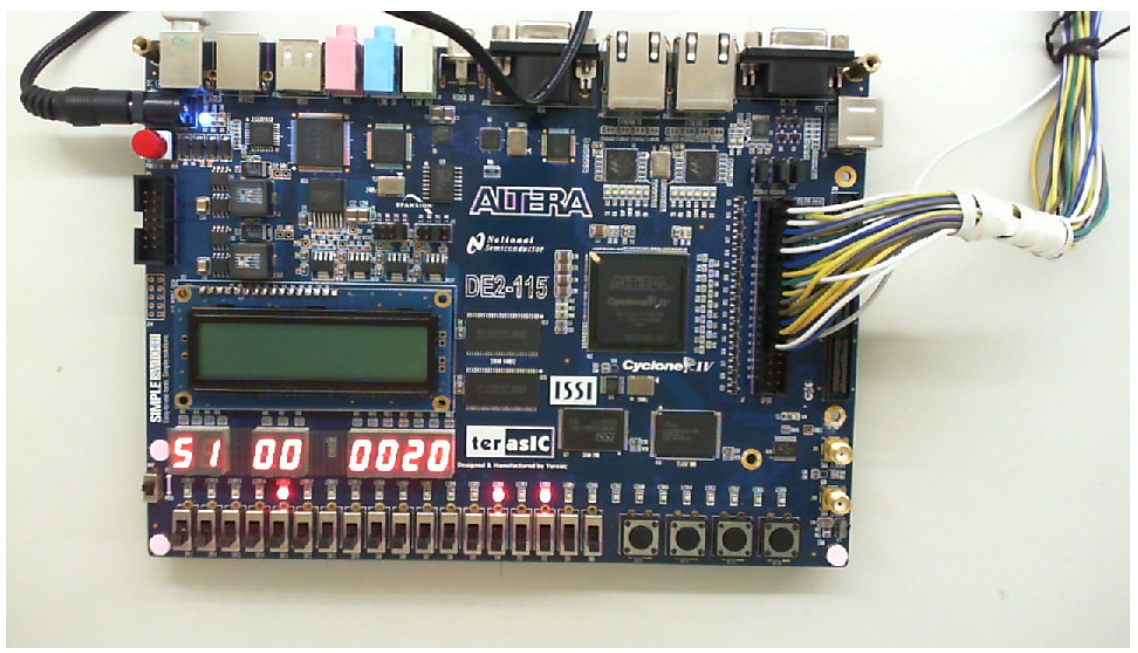
\includegraphics[scale=0.4]{imgs/Resultados/MDC_FPGA_Entrada1.png}
\legend{Fonte: O Autor }
\end{figure}

\begin{figure}[H]
\centering 
\caption{Número 5 obtido como resultado após o cálculo do máximo divisor comum} 
\label{fig:FPGAMDCSaida}
\graphicspath{ {./imgs/} } 
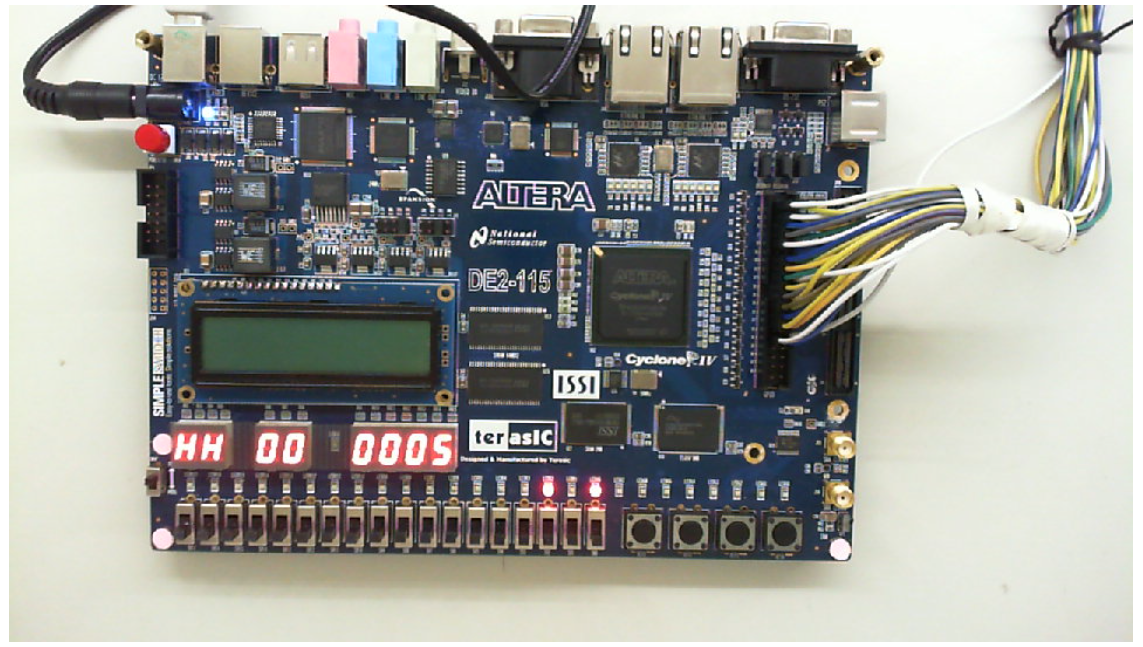
\includegraphics[scale=0.4]{imgs/Resultados/MDC_FPGA_Saida.png}
\legend{Fonte: O Autor }
\end{figure}

\section{Ordenação de Vetores}

\subsection{Código Fonte}

\begin{lstlisting} [language=C]
int vet[5];

int minloc (int a[], int low, int high){   
    int i; int x; int k;
    k = low;
    x = a[low];
    i = low + 1;
    while (i < high){
        if (a[i] < x){
            x = a[i];
            k = i;
        }
        i = i + 1;
    }
    return k;
}

void sort(int a[], int low, int high){   
    int i; int k;
    i = low;
    while (i < high-1){
        int t;
        
        k = minloc(a,i,high);
        t = a[k];
        a[k] = a[i];
        a[i] = t;
        i = i + 1;
    }
}

void main(void){	
    int i;
    
    i = 0;
    while(i < 5){
        vet[i] = input();
        i = i + 1;
    }
    
    sort(vet,0,5);
    
    while (1){
        output(vet[0]);
        output(vet[1]);
        output(vet[2]);
        output(vet[3]);
        output(vet[4]);
    }
}
\end{lstlisting}

\subsection{Código Intermediário}


% \usepackage{color}
% \usepackage{rotating}
% \usepackage{tabularray}
\begin{longtblr}[
  caption = {Código Intermediário},
  label = {tab: ResultadosSortIntermediario},
]{
  hlines,
  vlines,
}
ALLOC, vet, global, 5\\
FUN, INT, minloc, 3\\
ARG, VET, a, minloc\\
ARG, INT, low, minloc\\
ARG, INT, high, minloc\\
LOAD, \$t0, a, -\\
LOAD, \$t1, low, -\\
LOAD, \$t2, high, -\\
ALLOC, i, minloc, -\\
ALLOC, x, minloc, -\\
ALLOC, k, minloc, -\\
LOAD, \$t3, k, -\\
LOAD, \$t1, low, -\\
ASSIGN, \$t3, \$t1, -\\
STORE, k, \$t3, -\\
LOAD, \$t4, x, -\\
LOAD, \$t1, low, -\\
LOAD, \$t5, a, \$t1\\
ASSIGN, \$t4, \$t5, -\\
STORE, x, \$t4, -\\
LOAD, \$t6, i, -\\
LOAD, \$t1, low, -\\
LOADI, \$t7, 1, -\\
ADD, \$t1, \$t7, \$t8\\
ASSIGN, \$t6, \$t8, -\\
STORE, i, \$t6, -\\
LABEL, L1, -, -\\
LOAD, \$t6, i, -\\
LOAD, \$t2, high, -\\
LT, \$t6, \$t2, \$t9\\
IFF, \$t9, L2, -\\
LOAD, \$t6, i, -\\
LOAD, \$t10, a, \$t6\\
LOAD, \$t4, x, -\\
LT, \$t10, \$t4, \$t11\\
IFF, \$t11, L3, -\\
LOAD, \$t4, x, -\\
LOAD, \$t6, i, -\\
LOAD, \$t12, a, \$t6\\
ASSIGN, \$t4, \$t12, -\\
STORE, x, \$t4, -\\
LOAD, \$t3, k, -\\
LOAD, \$t6, i, -\\
ASSIGN, \$t3, \$t6, -\\
STORE, k, \$t3, -\\
LABEL, L3, -, -\\
LOAD, \$t6, i, -\\
LOAD, \$t6, i, -\\
LOADI, \$t13, 1, -\\
ADD, \$t6, \$t13, \$t14\\
ASSIGN, \$t6, \$t14, -\\
STORE, i, \$t6, -\\
GOTO, L1, -, -\\
LABEL, L2, -, -\\
LOAD, \$t3, k, -\\
RET, \$t3, -, -\\
GOTO, L0, -, -\\
LABEL, L0, -, -\\
END, minloc, -, -\\
FUN, VOID, sort, 3\\
ARG, VET, a, sort\\
ARG, INT, low, sort\\
ARG, INT, high, sort\\
LOAD, \$t15, a, -\\
LOAD, \$t16, low, -\\
LOAD, \$t17, high, -\\
ALLOC, i, sort, -\\
ALLOC, k, sort, -\\
LOAD, \$t18, i, -\\
LOAD, \$t16, low, -\\
ASSIGN, \$t18, \$t16, -\\
STORE, i, \$t18, -\\
LABEL, L6, -, -\\
LOAD, \$t18, i, -\\
LOAD, \$t17, high, -\\
LOADI, \$t19, 1, -\\
SUB, \$t17, \$t19, \$t20\\
LT, \$t18, \$t20, \$t21\\
IFF, \$t21, L7, -\\
ALLOC, t, sort, -\\
LOAD, \$t22, k, -\\
PARAM, \$t23, VET, a\\
LOAD, \$t18, i, -\\
PARAM, \$t18, INT, -\\
LOAD, \$t17, high, -\\
PARAM, \$t17, INT, -\\
CALL, minloc, 3, \$t24\\
ASSIGN, \$t22, \$t24, -\\
STORE, k, \$t22, -\\
LOAD, \$t25, t, -\\
LOAD, \$t22, k, -\\
LOAD, \$t5, a, \$t22\\
ASSIGN, \$t25, \$t5, -\\
STORE, t, \$t25, -\\
LOAD, \$t22, k, -\\
LOAD, \$t7, a, \$t22\\
LOAD, \$t18, i, -\\
LOAD, \$t8, a, \$t18\\
ASSIGN, \$t7, \$t8, -\\
STORE, a, \$t7, \$t22\\
LOAD, \$t18, i, -\\
LOAD, \$t9, a, \$t18\\
LOAD, \$t25, t, -\\
ASSIGN, \$t9, \$t25, -\\
STORE, a, \$t9, \$t18\\
LOAD, \$t18, i, -\\
LOAD, \$t18, i, -\\
LOADI, \$t10, 1, -\\
ADD, \$t18, \$t10, \$t11\\
ASSIGN, \$t18, \$t11, -\\
STORE, i, \$t18, -\\
GOTO, L6, -, -\\
LABEL, L7, -, -\\
LABEL, L5, -, -\\
END, sort, -, -\\
FUN, VOID, main, 0\\
ALLOC, i, main, -\\
LOAD, \$t12, i, -\\
ASSIGN, \$t12, \$t31, -\\
STORE, i, \$t12, -\\
LABEL, L9, -, -\\
LOAD, \$t12, i, -\\
LOADI, \$t13, 5, -\\
LT, \$t12, \$t13, \$t14\\
IFF, \$t14, L10, -\\
LOAD, \$t12, i, -\\
LOAD, \$t19, vet, \$t12\\
CALL, input, 0, \$t20\\
ASSIGN, \$t19, \$t20, -\\
STORE, vet, \$t19, \$t12\\
LOAD, \$t12, i, -\\
LOAD, \$t12, i, -\\
LOADI, \$t21, 1, -\\
ADD, \$t12, \$t21, \$t23\\
ASSIGN, \$t12, \$t23, -\\
STORE, i, \$t12, -\\
GOTO, L9, -, -\\
LABEL, L10, -, -\\
PARAM, \$t24, VET, vet\\
PARAM, \$t31, INT, -\\
LOADI, \$t5, 5, -\\
PARAM, \$t5, INT, -\\
CALL, sort, 3, -\\
LABEL, L11, -, -\\
LOADI, \$t7, 1, -\\
IFF, \$t7, L12, -\\
LOAD, \$t8, vet, \$t31\\
PARAM, \$t8, INT, -\\
CALL, output, 1, -\\
LOADI, \$t9, 1, -\\
LOAD, \$t10, vet, \$t9\\
PARAM, \$t10, INT, -\\
CALL, output, 1, -\\
LOADI, \$t11, 2, -\\
LOAD, \$t13, vet, \$t11\\
PARAM, \$t13, INT, -\\
CALL, output, 1, -\\
LOADI, \$t14, 3, -\\
LOAD, \$t19, vet, \$t14\\
PARAM, \$t19, INT, -\\
CALL, output, 1, -\\
LOADI, \$t20, 4, -\\
LOAD, \$t21, vet, \$t20\\
PARAM, \$t21, INT, -\\
CALL, output, 1, -\\
GOTO, L11, -, -\\
LABEL, L12, -, -\\
LABEL, L8, -, -\\
END, main, -, -\\
HALT, -, -, -
\end{longtblr}
\legend{Fonte: O Autor}

\subsection{Código Assembly e Binário}

% \usepackage{color}
% \usepackage{rotating}
% \usepackage{tabularray}
% \usepackage{color}
% \usepackage{rotating}
% \usepackage{tabularray}
\begin{longtblr}[
  caption = {Geração dos códigos assembly e binário},
  label = {tab:ResultadosSortBin},
]{
  hlines,
  vlines,
}
j main & 00001000000000000000000010001101\\
minloc: & 00000011111111111111100000100000\\
sw \$ra 4(\$fp) & 10101111101111100000000000000100\\
lw \$t0 0(\$fp) & 10001111101000000000000000000000\\
lw \$t1 1(\$fp) & 10001111101000010000000000000001\\
lw \$t2 2(\$fp) & 10001111101000100000000000000010\\
lw \$t3 11(\$fp) & 10001111101000110000000000001011\\
lw \$t1 1(\$fp) & 10001111101000010000000000000001\\
add \$t3 \$zero \$t1 & 00000011111000010001100000100000\\
sw \$t3 11(\$fp) & 10101111101000110000000000001011\\
lw \$t4 10(\$fp) & 10001111101001000000000000001010\\
lw \$t1 1(\$fp) & 10001111101000010000000000000001\\
lw \$temp 0(\$fp) & 10001111101110110000000000000000\\
add \$temp \$temp \$t1 & 00000011011000011101100000100000\\
lw \$t5 0(\$temp) & 10001111011001010000000000000000\\
add \$t4 \$zero \$t5 & 00000011111001010010000000100000\\
sw \$t4 10(\$fp) & 10101111101001000000000000001010\\
lw \$t6 9(\$fp) & 10001111101001100000000000001001\\
lw \$t1 1(\$fp) & 10001111101000010000000000000001\\
ori \$t7 \$zero 1 & 00110111111001110000000000000001\\
add \$t8 \$t1 \$t7 & 00000000001001110100000000100000\\
add \$t6 \$zero \$t8 & 00000011111010000011000000100000\\
sw \$t6 9(\$fp) & 10101111101001100000000000001001\\
Label 1: & 00000011111111111111100000100000\\
lw \$t6 9(\$fp) & 10001111101001100000000000001001\\
lw \$t2 2(\$fp) & 10001111101000100000000000000010\\
slt \$t9 \$t6 \$t2 & 00000000110000100100100000101010\\
beq \$t9 \$zero Label 2 & 00010011111010010000000000110110\\
lw \$t6 9(\$fp) & 10001111101001100000000000001001\\
lw \$temp 0(\$fp) & 10001111101110110000000000000000\\
add \$temp \$temp \$t6 & 00000011011001101101100000100000\\
lw \$t10 0(\$temp) & 10001111011010100000000000000000\\
lw \$t4 10(\$fp) & 10001111101001000000000000001010\\
slt \$t11 \$t10 \$t4 & 00000001010001000101100000101010\\
beq \$t11 \$zero Label 3 & 00010011111010110000000000101110\\
lw \$t4 10(\$fp) & 10001111101001000000000000001010\\
lw \$t6 9(\$fp) & 10001111101001100000000000001001\\
lw \$temp 0(\$fp) & 10001111101110110000000000000000\\
add \$temp \$temp \$t6 & 00000011011001101101100000100000\\
lw \$t12 0(\$temp) & 10001111011011000000000000000000\\
add \$t4 \$zero \$t12 & 00000011111011000010000000100000\\
sw \$t4 10(\$fp) & 10101111101001000000000000001010\\
lw \$t3 11(\$fp) & 10001111101000110000000000001011\\
lw \$t6 9(\$fp) & 10001111101001100000000000001001\\
add \$t3 \$zero \$t6 & 00000011111001100001100000100000\\
sw \$t3 11(\$fp) & 10101111101000110000000000001011\\
Label 3: & 00000011111111111111100000100000\\
lw \$t6 9(\$fp) & 10001111101001100000000000001001\\
lw \$t6 9(\$fp) & 10001111101001100000000000001001\\
ori \$t13 \$zero 1 & 00110111111011010000000000000001\\
add \$t14 \$t6 \$t13 & 00000000110011010111000000100000\\
add \$t6 \$zero \$t14 & 00000011111011100011000000100000\\
sw \$t6 9(\$fp) & 10101111101001100000000000001001\\
j Label 1 & 00001000000000000000000000010111\\
Label 2: & 00000011111111111111100000100000\\
lw \$t3 11(\$fp) & 10001111101000110000000000001011\\
lw \$temp 3(\$fp) & 10001111101110110000000000000011\\
sw \$t3 2(\$temp) & 10101111011000110000000000000010\\
j Label 0 & 00001000000000000000000000111011\\
Label 0: & 00000011111111111111100000100000\\
lw \$ra 4(\$fp) & 10001111101111100000000000000100\\
jr \$zero \$ra \$zero & 00000011110111111111100000001000\\
sort: & 00000011111111111111100000100000\\
sw \$ra 4(\$fp) & 10101111101111100000000000000100\\
lw \$t15 0(\$fp) & 10001111101011110000000000000000\\
lw \$t16 1(\$fp) & 10001111101100000000000000000001\\
lw \$t17 2(\$fp) & 10001111101100010000000000000010\\
lw \$t18 9(\$fp) & 10001111101100100000000000001001\\
lw \$t16 1(\$fp) & 10001111101100000000000000000001\\
add \$t18 \$zero \$t16 & 00000011111100001001000000100000\\
sw \$t18 9(\$fp) & 10101111101100100000000000001001\\
Label 6: & 00000011111111111111100000100000\\
lw \$t18 9(\$fp) & 10001111101100100000000000001001\\
lw \$t17 2(\$fp) & 10001111101100010000000000000010\\
ori \$t19 \$zero 1 & 00110111111100110000000000000001\\
sub \$t20 \$t17 \$t19 & 00000010001100111010000000100010\\
slt \$t21 \$t18 \$t20 & 00000010010101001010100000101010\\
beq \$t21 \$zero Label 7 & 00010011111101010000000010001001\\
lw \$t22 10(\$fp) & 10001111101101100000000000001010\\
lw \$t23 0(\$fp) & 10001111101101110000000000000000\\
sw \$t23 0(\$pilha) & 10101111010101110000000000000000\\
lw \$t18 9(\$fp) & 10001111101100100000000000001001\\
sw \$t18 1(\$pilha) & 10101111010100100000000000000001\\
lw \$t17 2(\$fp) & 10001111101100010000000000000010\\
sw \$t17 2(\$pilha) & 10101111010100010000000000000010\\
lw \$temp 2(\$pilha) & 10001111010110110000000000000010\\
sw \$temp 3(\$sp) & 10101111100110110000000000000011\\
lw \$temp 1(\$pilha) & 10001111010110110000000000000001\\
sw \$temp 2(\$sp) & 10101111100110110000000000000010\\
lw \$temp 0(\$pilha) & 10001111010110110000000000000000\\
sw \$temp 1(\$sp) & 10101111100110110000000000000001\\
add \$temp \$fp \$zero & 00000011101111111101100000100000\\
addi \$temp \$temp 3 & 00100011011110110000000000000011\\
sw \$temp 4(\$sp) & 10101111100110110000000000000100\\
addi \$fp \$fp 25 & 00100011101111010000000000011001\\
addi \$sp \$sp 25 & 00100011100111000000000000011001\\
jal minloc & 00001100000000000000000000000001\\
subi \$fp \$fp 25 & 00100111101111010000000000011001\\
subi \$sp \$sp 25 & 00100111100111000000000000011001\\
lw \$t24 5(\$fp) & 10001111101110000000000000000101\\
add \$t22 \$zero \$t24 & 00000011111110001011000000100000\\
sw \$t22 10(\$fp) & 10101111101101100000000000001010\\
lw \$t25 11(\$fp) & 10001111101110010000000000001011\\
lw \$t22 10(\$fp) & 10001111101101100000000000001010\\
lw \$temp 0(\$fp) & 10001111101110110000000000000000\\
add \$temp \$temp \$t22 & 00000011011101101101100000100000\\
lw \$t5 0(\$temp) & 10001111011001010000000000000000\\
add \$t25 \$zero \$t5 & 00000011111001011100100000100000\\
sw \$t25 11(\$fp) & 10101111101110010000000000001011\\
lw \$t22 10(\$fp) & 10001111101101100000000000001010\\
lw \$temp 0(\$fp) & 10001111101110110000000000000000\\
add \$temp \$temp \$t22 & 00000011011101101101100000100000\\
lw \$t7 0(\$temp) & 10001111011001110000000000000000\\
lw \$t18 9(\$fp) & 10001111101100100000000000001001\\
lw \$temp 0(\$fp) & 10001111101110110000000000000000\\
add \$temp \$temp \$t18 & 00000011011100101101100000100000\\
lw \$t8 0(\$temp) & 10001111011010000000000000000000\\
add \$t7 \$zero \$t8 & 00000011111010000011100000100000\\
lw \$temp 0(\$fp) & 10001111101110110000000000000000\\
add \$temp \$temp \$t22 & 00000011011101101101100000100000\\
sw \$t7 0(\$temp) & 10101111011001110000000000000000\\
lw \$t18 9(\$fp) & 10001111101100100000000000001001\\
lw \$temp 0(\$fp) & 10001111101110110000000000000000\\
add \$temp \$temp \$t18 & 00000011011100101101100000100000\\
lw \$t9 0(\$temp) & 10001111011010010000000000000000\\
lw \$t25 11(\$fp) & 10001111101110010000000000001011\\
add \$t9 \$zero \$t25 & 00000011111110010100100000100000\\
lw \$temp 0(\$fp) & 10001111101110110000000000000000\\
add \$temp \$temp \$t18 & 00000011011100101101100000100000\\
sw \$t9 0(\$temp) & 10101111011010010000000000000000\\
lw \$t18 9(\$fp) & 10001111101100100000000000001001\\
lw \$t18 9(\$fp) & 10001111101100100000000000001001\\
ori \$t10 \$zero 1 & 00110111111010100000000000000001\\
add \$t11 \$t18 \$t10 & 00000010010010100101100000100000\\
add \$t18 \$zero \$t11 & 00000011111010111001000000100000\\
sw \$t18 9(\$fp) & 10101111101100100000000000001001\\
j Label 6 & 00001000000000000000000001000111\\
Label 7: & 00000011111111111111100000100000\\
Label 5: & 00000011111111111111100000100000\\
lw \$ra 4(\$fp) & 10001111101111100000000000000100\\
jr \$zero \$ra \$zero & 00000011110111111111100000001000\\
main: & 00000011111111111111100000100000\\
ori \$fp \$zero 5 & 00110111111111010000000000000101\\
ori \$sp \$zero 29 & 00110111111111000000000000011101\\
ori \$pilha \$zero 1000 & 00110111111110100000001111101000\\
lw \$t12 6(\$fp) & 10001111101011000000000000000110\\
add \$t12 \$zero \$zero & 00000011111111110110000000100000\\
sw \$t12 6(\$fp) & 10101111101011000000000000000110\\
Label 9: & 00000011111111111111100000100000\\
lw \$t12 6(\$fp) & 10001111101011000000000000000110\\
ori \$t13 \$zero 5 & 00110111111011010000000000000101\\
slt \$t14 \$t12 \$t13 & 00000001100011010111000000101010\\
beq \$t14 \$zero Label 10 & 00010011111011100000000010101001\\
lw \$t12 6(\$fp) & 10001111101011000000000000000110\\
addi \$temp \$zero 0 & 00100011111110110000000000000000\\
add \$temp \$temp \$t12 & 00000011011011001101100000100000\\
lw \$t19 0(\$temp) & 10001111011100110000000000000000\\
in \$t20 \$zero 0 & 01111111111101000000000000000000\\
add \$t19 \$zero \$t20 & 00000011111101001001100000100000\\
addi \$temp \$zero 0 & 00100011111110110000000000000000\\
add \$temp \$temp \$t12 & 00000011011011001101100000100000\\
sw \$t19 0(\$temp) & 10101111011100110000000000000000\\
lw \$t12 6(\$fp) & 10001111101011000000000000000110\\
lw \$t12 6(\$fp) & 10001111101011000000000000000110\\
ori \$t21 \$zero 1 & 00110111111101010000000000000001\\
add \$t23 \$t12 \$t21 & 00000001100101011011100000100000\\
add \$t12 \$zero \$t23 & 00000011111101110110000000100000\\
sw \$t12 6(\$fp) & 10101111101011000000000000000110\\
j Label 9 & 00001000000000000000000010010100\\
Label 10: & 00000011111111111111100000100000\\
addi \$t24 \$zero 0 & 00100011111110000000000000000000\\
sw \$t24 0(\$pilha) & 10101111010110000000000000000000\\
sw \$zero 1(\$pilha) & 10101111010111110000000000000001\\
ori \$t5 \$zero 5 & 00110111111001010000000000000101\\
sw \$t5 2(\$pilha) & 10101111010001010000000000000010\\
lw \$temp 2(\$pilha) & 10001111010110110000000000000010\\
sw \$temp 3(\$sp) & 10101111100110110000000000000011\\
lw \$temp 1(\$pilha) & 10001111010110110000000000000001\\
sw \$temp 2(\$sp) & 10101111100110110000000000000010\\
lw \$temp 0(\$pilha) & 10001111010110110000000000000000\\
sw \$temp 1(\$sp) & 10101111100110110000000000000001\\
add \$temp \$fp \$zero & 00000011101111111101100000100000\\
addi \$temp \$temp 0 & 00100011011110110000000000000000\\
sw \$temp 4(\$sp) & 10101111100110110000000000000100\\
addi \$fp \$fp 25 & 00100011101111010000000000011001\\
addi \$sp \$sp 25 & 00100011100111000000000000011001\\
jal sort & 00001100000000000000000000111110\\
subi \$fp \$fp 25 & 00100111101111010000000000011001\\
subi \$sp \$sp 25 & 00100111100111000000000000011001\\
Label 11: & 00000011111111111111100000100000\\
ori \$t7 \$zero 1 & 00110111111001110000000000000001\\
beq \$t7 \$zero Label 12 & 00010011111001110000000011100011\\
addi \$temp \$zero 0 & 00100011111110110000000000000000\\
add \$temp \$temp \$zero & 00000011011111111101100000100000\\
lw \$t8 0(\$temp) & 10001111011010000000000000000000\\
sw \$t8 0(\$pilha) & 10101111010010000000000000000000\\
lw \$temp 0(\$pilha) & 10001111010110110000000000000000\\
out \$zero \$temp 0 & 01111011011111110000000000000000\\
ori \$t9 \$zero 1 & 00110111111010010000000000000001\\
addi \$temp \$zero 0 & 00100011111110110000000000000000\\
add \$temp \$temp \$t9 & 00000011011010011101100000100000\\
lw \$t10 0(\$temp) & 10001111011010100000000000000000\\
sw \$t10 0(\$pilha) & 10101111010010100000000000000000\\
lw \$temp 0(\$pilha) & 10001111010110110000000000000000\\
out \$zero \$temp 0 & 01111011011111110000000000000000\\
ori \$t11 \$zero 2 & 00110111111010110000000000000010\\
addi \$temp \$zero 0 & 00100011111110110000000000000000\\
add \$temp \$temp \$t11 & 00000011011010111101100000100000\\
lw \$t13 0(\$temp) & 10001111011011010000000000000000\\
sw \$t13 0(\$pilha) & 10101111010011010000000000000000\\
lw \$temp 0(\$pilha) & 10001111010110110000000000000000\\
out \$zero \$temp 0 & 01111011011111110000000000000000\\
ori \$t14 \$zero 3 & 00110111111011100000000000000011\\
addi \$temp \$zero 0 & 00100011111110110000000000000000\\
add \$temp \$temp \$t14 & 00000011011011101101100000100000\\
lw \$t19 0(\$temp) & 10001111011100110000000000000000\\
sw \$t19 0(\$pilha) & 10101111010100110000000000000000\\
lw \$temp 0(\$pilha) & 10001111010110110000000000000000\\
out \$zero \$temp 0 & 01111011011111110000000000000000\\
ori \$t20 \$zero 4 & 00110111111101000000000000000100\\
addi \$temp \$zero 0 & 00100011111110110000000000000000\\
add \$temp \$temp \$t20 & 00000011011101001101100000100000\\
lw \$t21 0(\$temp) & 10001111011101010000000000000000\\
sw \$t21 0(\$pilha) & 10101111010101010000000000000000\\
lw \$temp 0(\$pilha) & 10001111010110110000000000000000\\
out \$zero \$temp 0 & 01111011011111110000000000000000\\
j Label 11 & 00001000000000000000000010111101\\
Label 12: & 00000011111111111111100000100000\\
Label 8: & 00000011111111111111100000100000\\
halt \$zero & 11111111111111111111111111111111
\end{longtblr}

\legend{Fonte: O Autor}
%-------------------- Considerações Finais ---------------------
\chapter{Considerações Finais}
A realização de projetos em arquitetura e organização de computadores são de extrema importância para conseguirmos colocar em prática muito dos conceitos teóricos vistos em aula, permitindo uma evolução do pensamento técnico do aluno. Como engenheiros da computação, é imprescindível que sejamos capazes de planejar, desde o \emph{design} de uma arquitetura de processador, até a sua devida implementação. Além disso, ao sair de uma zona de conforto, o aluno deve buscar os conhecimentos teóricos que faltam para conseguir realizar tal desafio.

Além disso, ao projetar um compilador desde sua fase de análise até a de síntese é possível entender aprofundadamente como o programa que é utilizado diariamente pelos estudantes na graduação de computação realiza a analise e gera os códigos executáveis dos computadores atualmente. O desenvolvimento desse \emph{software} é extremamente trabalhoso e demanda do aluno a conexão e melhoramento de diversos outros projetos realizados em disciplinas passadas, porém o seu resultado é grandioso para o desenvolvimento das habilidades de programação e de entendimento do que o código escrito na linguagem de programação realmente significa para a máquina.

Por fim, nota-se após a realização de testes, com a utilização da placa FPGA disponibilizada de forma online e presencial, que o compilador consegue transformar o código de alto nível para código binário capaz de efetuar as operações pedidas pelo usuário, considerando também as limitações impostas pelo próprio processador e pela linguagem de programação C-.

% ---
% Finaliza a parte no bookmark do PDF
% para que se inicie o bookmark na raiz
% e adiciona espaço de parte no Sumário
% ---
\phantompart


% ----------------------------------------------------------
% ELEMENTOS PÓS-TEXTUAIS
% ----------------------------------------------------------
\postextual

% ----------------------------------------------------------
% Referências bibliográficas
% ----------------------------------------------------------
\bibliography{referencias}



\end{document}
